%% Hanford investigations

%% TCS schematic for LIGO Hanford for O3
%% TCS pre-loading
 %% Current methodology for tuning TCS
  %% Detail Hanford's methods
 %% Increasing RH tuning speed


%As shown in Chapter 1,  

\section{Motivation}
As seen in ~\autoref{sec:detcon}, increasing detector input power leads to a direct sensitivity increase to gravitational waves. And even using optics with ultra-low absorption ($\approx 400 \; \mathrm{ppb} \pm 150 \; \mathrm{ppb}$ \textcolor{red}{alog ? or point absorber paper}) there still are induced thermo-optic effects with a designed circulating arm power of 750 kW in the Fabry-P\'{e}rot cavity arms. Predicted thermal aberrations produced include a substrate lens with relatively smaller lensing from the differential HR surface curvature. This time varying optical path length change integrated over the carrier phasefront produces mode mismatch and contributes to the accumulated optical loss throughought GWDs which reduces sensitivity two-fold: by loss of readout power, and reduced efficacy to produce squeezed light states in lowering the detector quantum noise limit.
\\
During O3a the LIGO Hanford observatory increased circulating arm power beyond 180 kW; emphasizing importance on properly tuned thermal compensation in O3 to avert arm-cavity/carrier-beam mode mismatch. Detailed in this chapter is a summary of related comissioning efforts at LHO to prepare and preserve interferometer mode matching including but not exclusive to: a primer on the ALIGO adaptive optics schema (TCS), citations on the initial computed O3 TCS pre-load, the development and implementation of real-time digital filtering for an improved ring heater actuation response by a factor of $\approx 6$, and the impacts of high absorption points aka point absorbers discovered on arm cavity test masses along with the some efforts to mitigate them.

\subsection{Thermal Compensation System}
High power beams, even propogated by ultra low absorption mirror substrates and coatings, can impart a surface pressure that imposes non-negligible thermo-optic distortions via thermo-refractive and thermo-elastic effects~\cite{hellovinet:1990}. The ALIGO adaptive optic system is intended to address the problem of dynamic mode mismatch in high power interferometry; as high power operation is a requirement in reaching designed sensitivity. Comprised of a feedback control system that uses four Hartmann wavefront sensors (HWS) combined with thermal actuators of two varieties: annular ring heaters and CO2 lasers. 

\subsubsection{Actuation}
Both ITMs and ETMs (Fabry-P\'{e}rot arm cavity mirrors) are strategically monitored for differential lensing, but both are not prescribed equal actuation treatment. All arm cavity mirrors do posses negative lens ring heater actuation in the form of a wound nichrome wire annulus that outlines the outer barrel of the mirror substrate; while CO2 lasers, though not imaged onto the ITMs directly \footnote{Decouples CO2 laser noise from the highly sensitive FP input test mass position}, are instead imaged onto a compensation plate (CP) placed promptly before the FP arm input coupling mirror ~\cite{brooks:aigwd2019}.

\subsubsection{Sensing Optical Path Distortion}
Quantifying thermal distortion from both carrier as well as thermal actuators is performed with a set of four Hartmann wavefront sensors; each one measuring differential optical path distortion at each FP cavity test masses. The sensor probe beams \footnote{Differing wavelengths of 800 nm and 833 nm are chosen for the X and Y arms in order to mitigate crosstalk between HWS chains and other auxilary systems} make a double pass through the test mass mirror substrate for all arm cavity mirrors and map the HR mirror surface; while the two input test mass sensors at the interferometer vertex make an additional double pass through the compensation plate (CP) ~\cite{aasi:2015}.

\subsection{Transient thermo-optic response}
\begin{figure}[H]
  \centering
  \begin{subcaptiongroup}
	  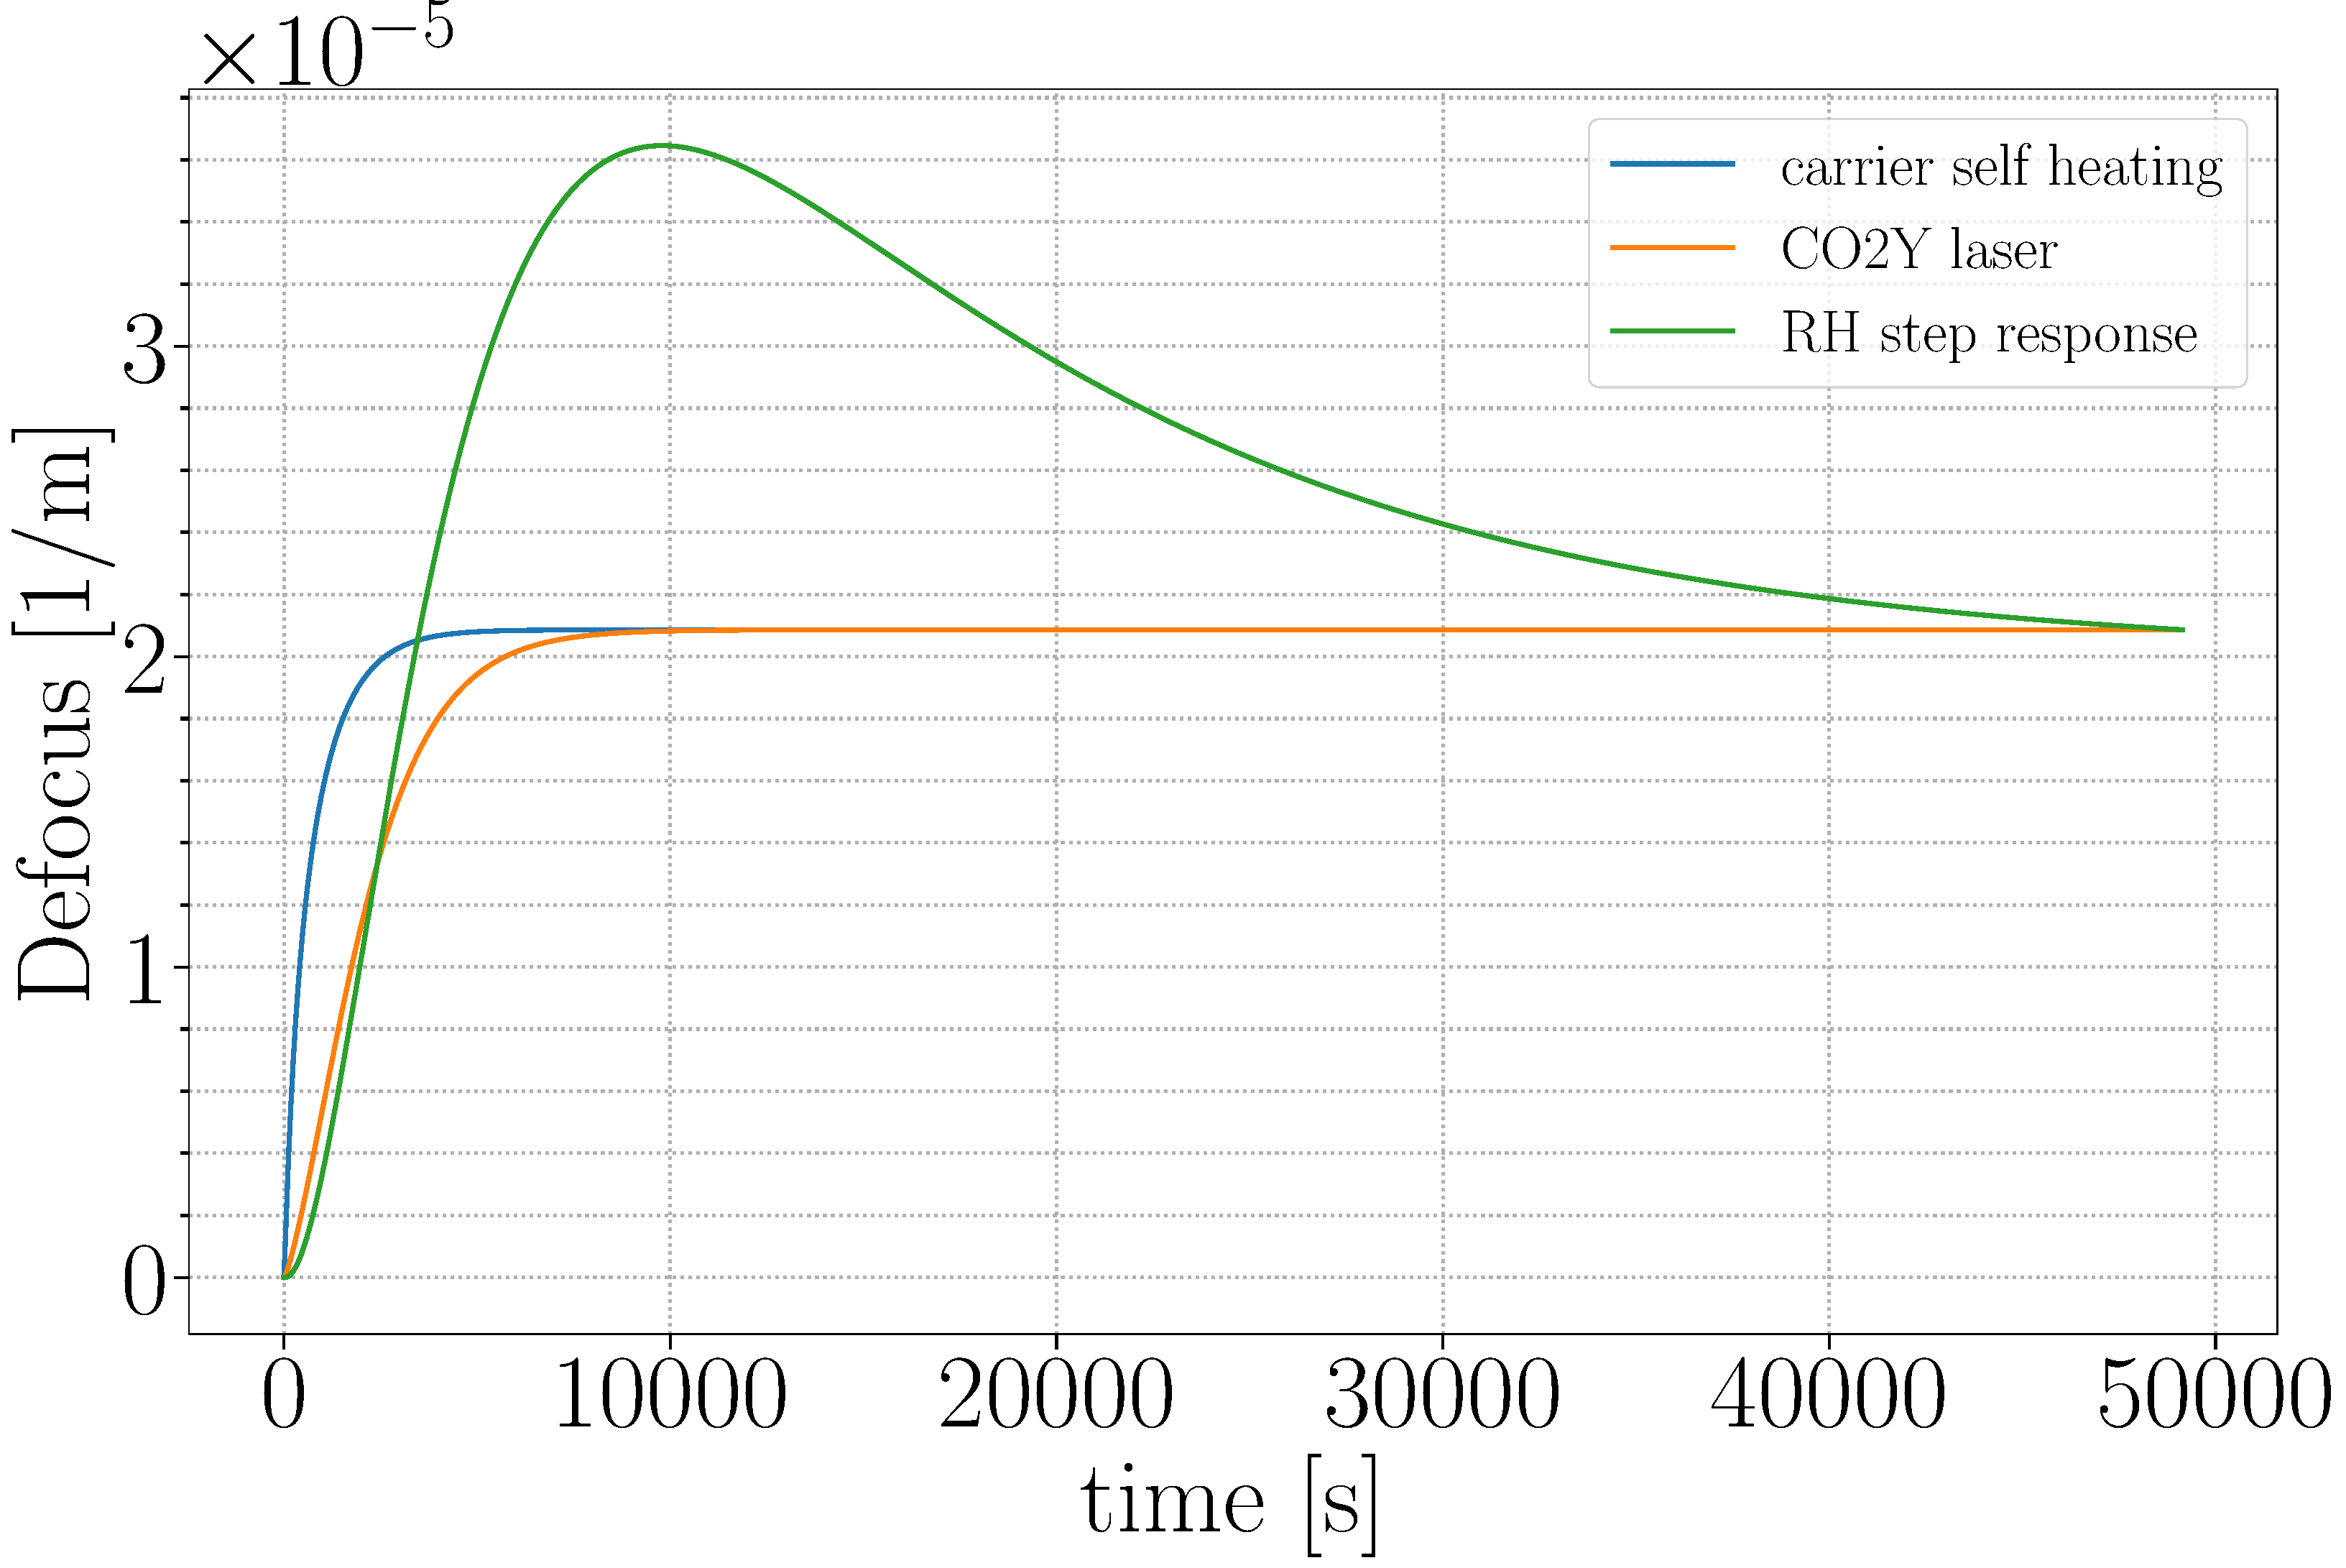
\includegraphics[width=\textwidth]{TCS/TCS_resp_sim.pdf}
	  \phantomcaption\label{TO_response}
  \end{subcaptiongroup}
  \captionsetup{subrefformat=parens}
  \hfill
  \caption{Transient defocus responses computed from carrier beam self heating and TCS actuation best fit filters (central CO2 laser heating and annular ring heating) \autoref{}.} 
\label{fig:thermooptic_response}
\end{figure}
The thermo-optic time constant of central carrier beam self-heating is similar to that seen from CO2 laser / CP central actuation, though demonstrably different from annular ring heating. Because of this, LHO applies central CO2 heating and static annular ring heating to a power level that respectively mimics and actuates for projected thermal deformation from circulating resonant carrier in the Fabry-Perot arm cavities. Once DRFPMI coupled cavities are configured or ``locked'', the input carrier power is gradually increased while CO2 laser power is simultaneously decreased in order to mitigate any possible differential thermo-optic response from the arm cavity test masses when reaching maximum power.

\begin{figure}[H]
	\begin{subcaptiongroup}
		\centering
		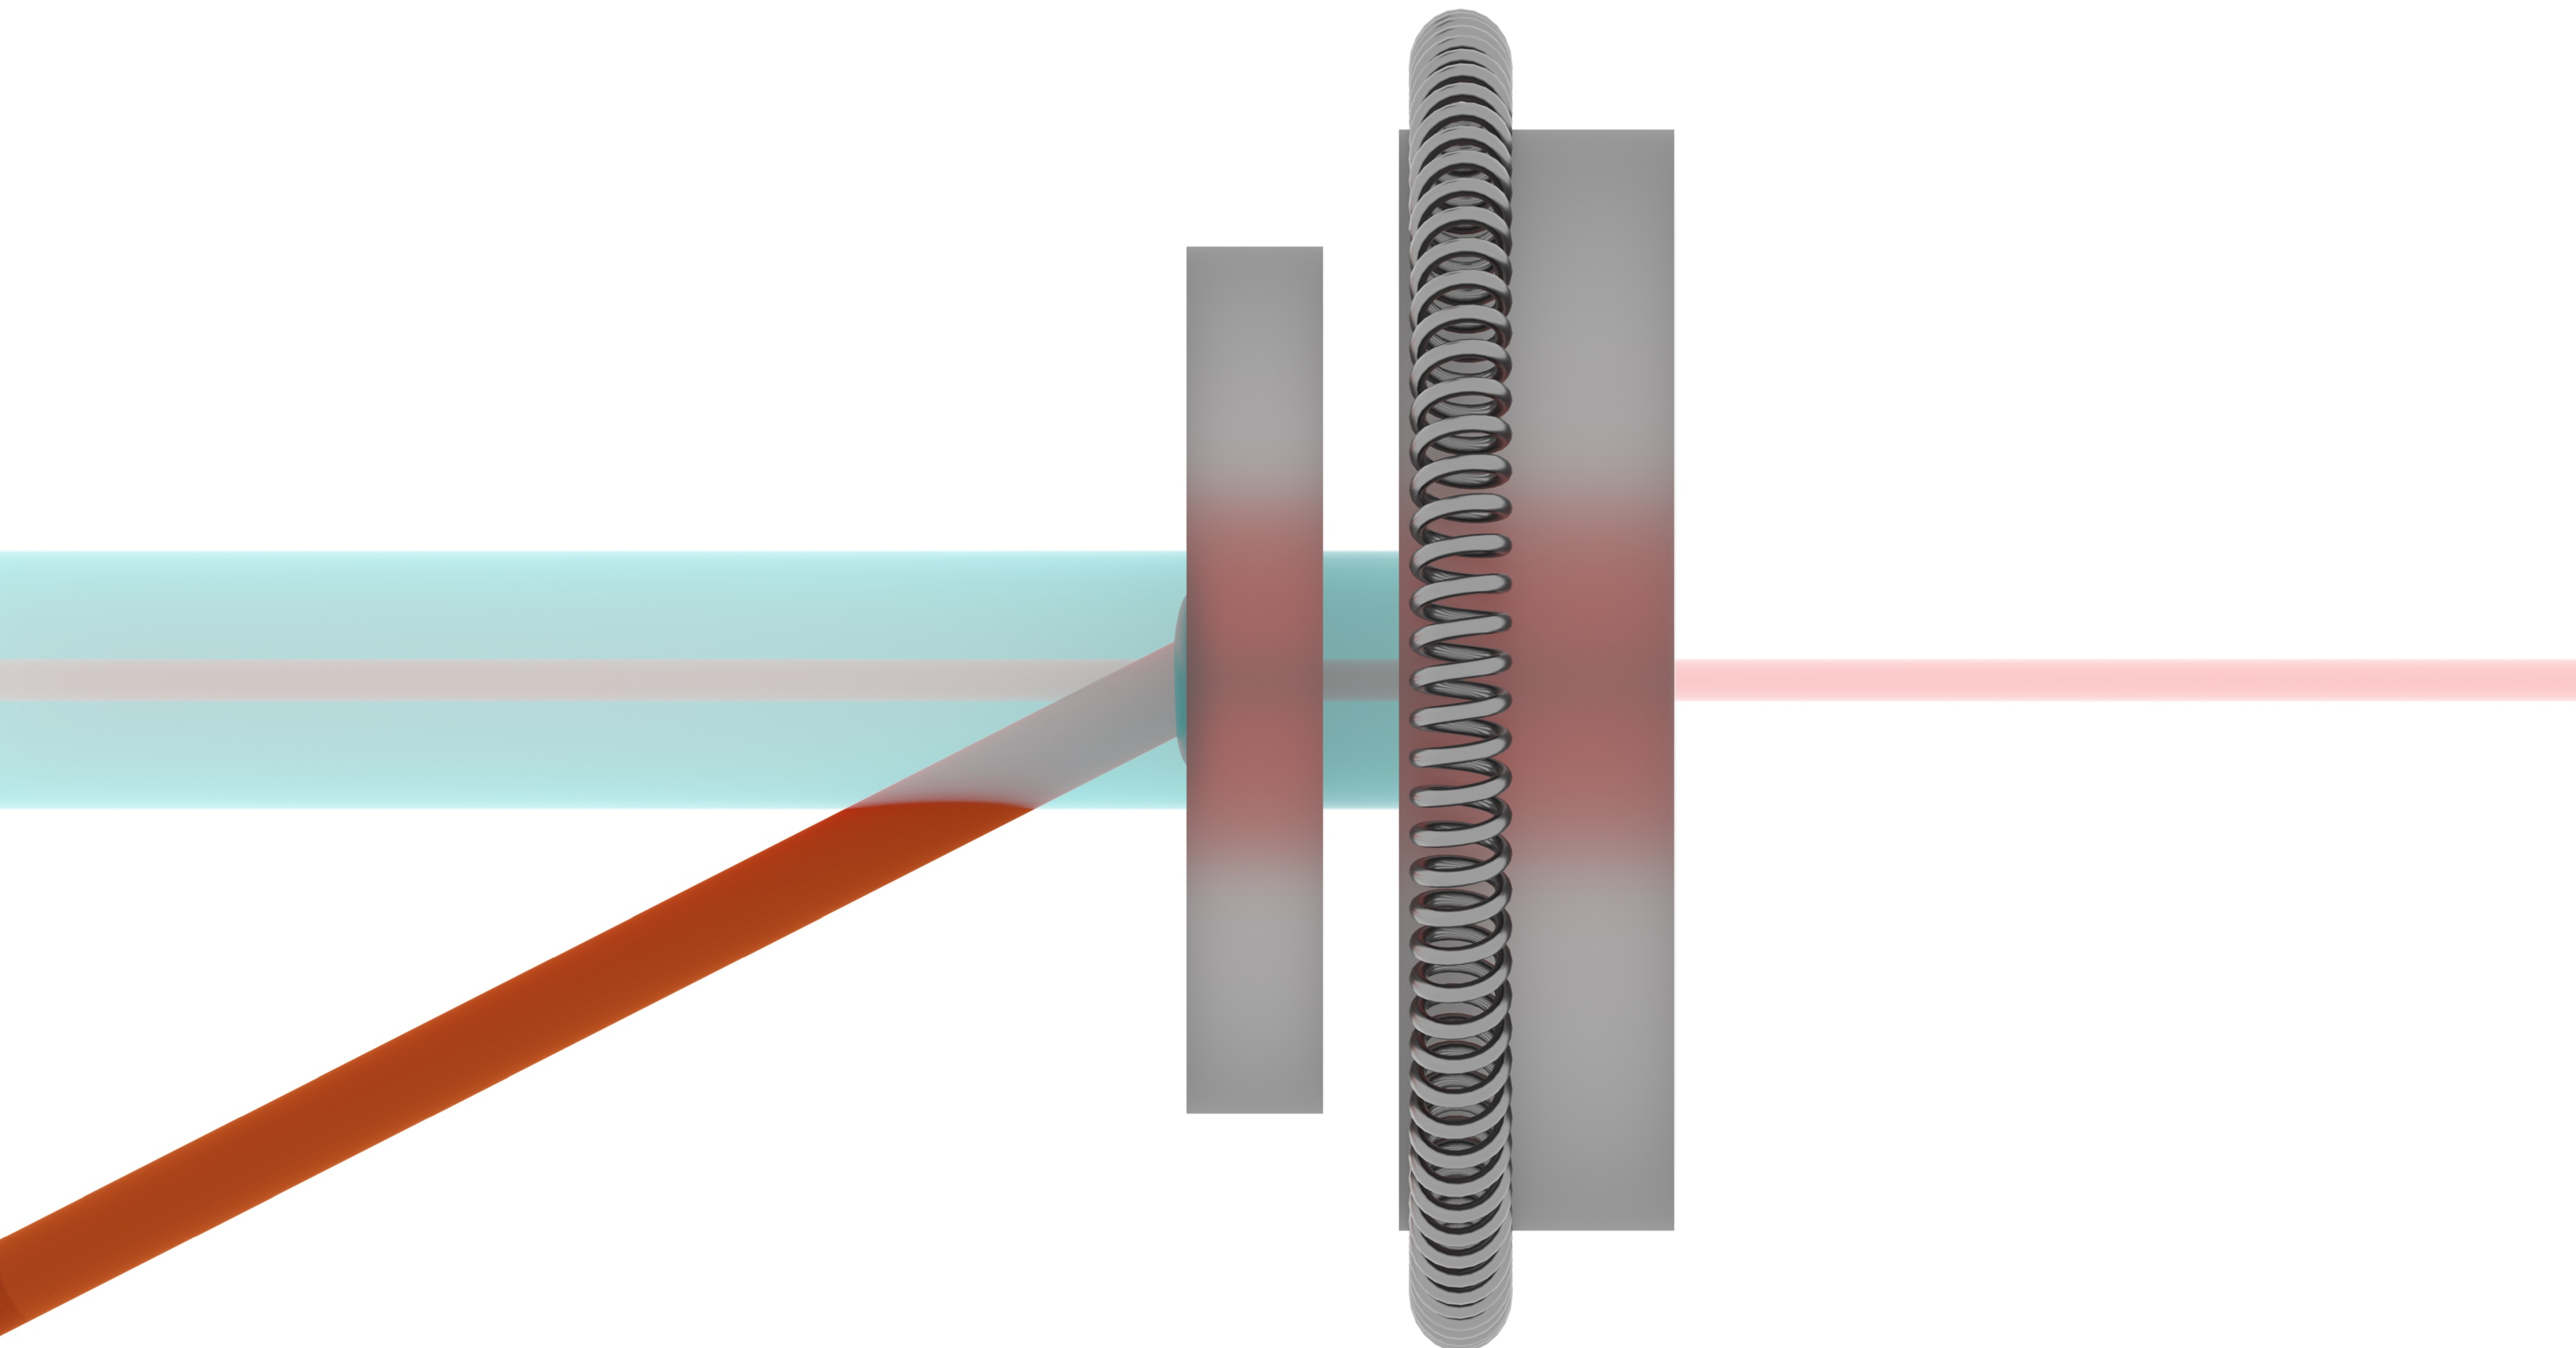
\includegraphics[width=.6\textwidth]{TCS/ITMYarminp/annotated/max/ITMYinp_lowcirc.pdf}
		\caption{CO2 actuator set to replicate projected carrier thermo-optic response, with an off resonance circulating beam.}\label{subfig:TCSinp_lowcirc}
%		\caption{(A) The incident carrier beam and (B) }\label{TCSinp_lowcirc}
		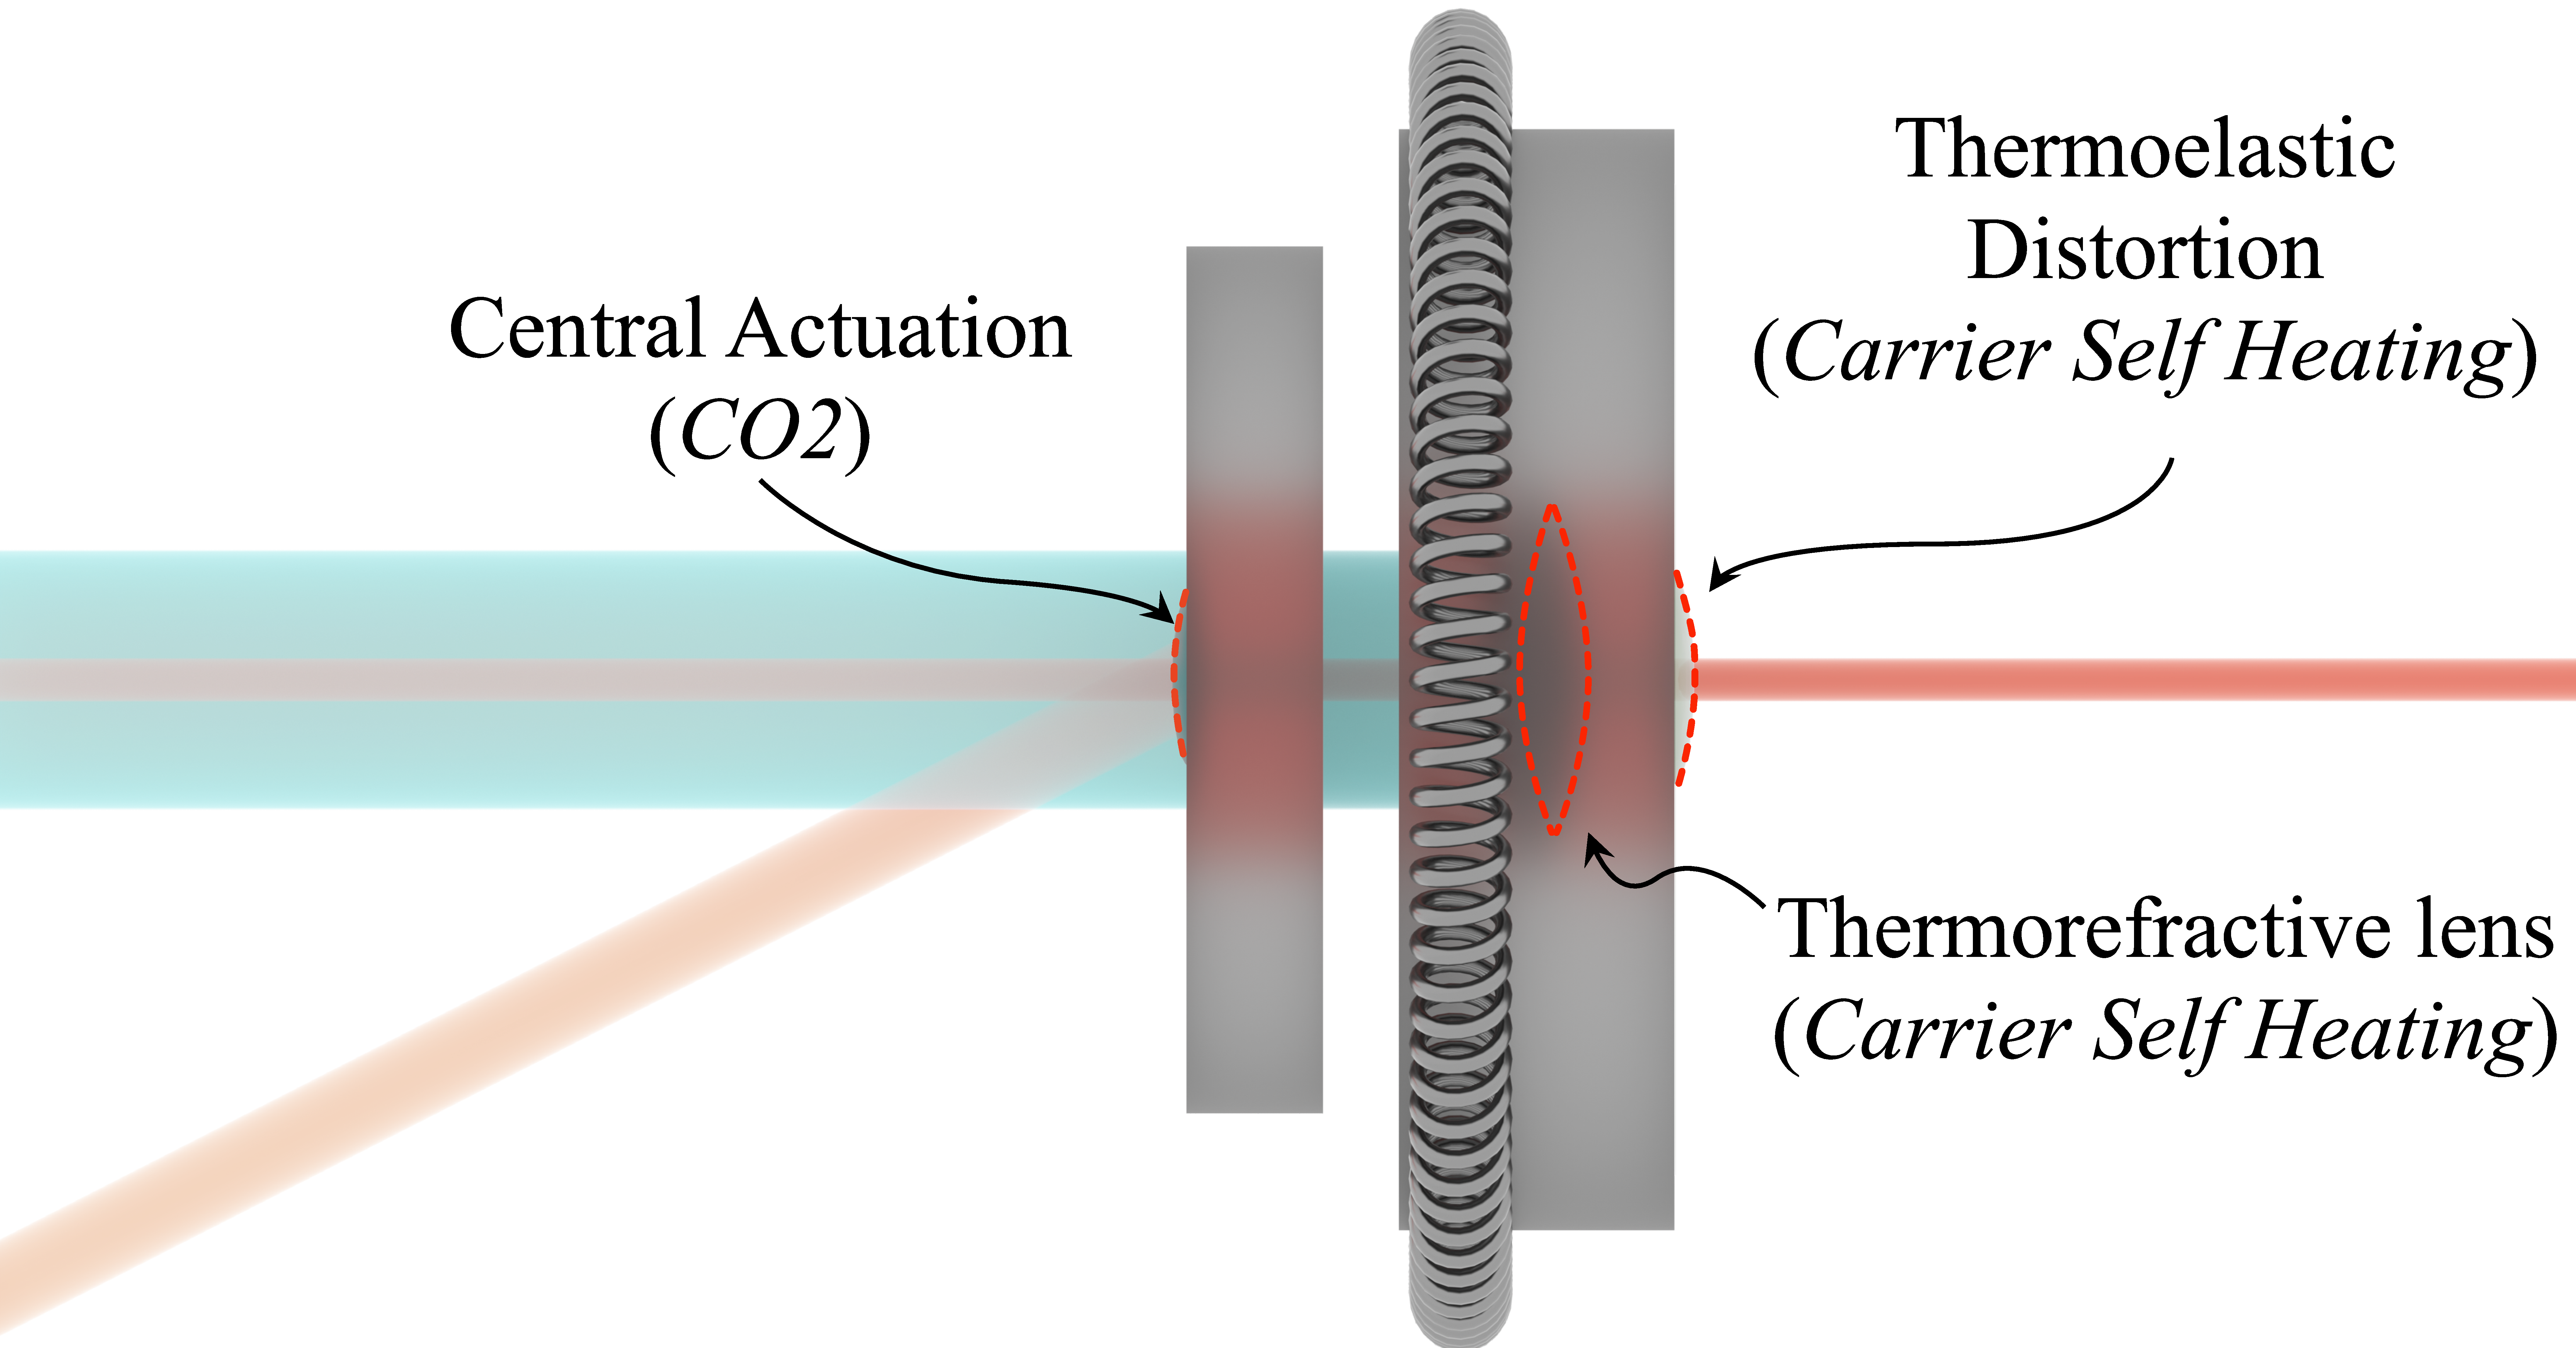
\includegraphics[width=.6\textwidth]{TCS/ITMYarminp/annotated/max/ITMYinp_intermcirc.pdf}
		\caption{Arm cavity resonance, with reduced CO2 central actuation power and increased arm cavity input power. The uniform thermo-optic distortion from the high power circulating carrier imposes a differential thermo-refractive lens and thermo-elastic HR surface change to the ITM, placing a low upper to the circulating power limit without annular ring heater actuation.}\label{subfig:TCSinp_intcirc}
%		\caption{Arm cavity resonance, with reduced CO2 central actuation power and increased arm cavity input power. The uniform thermo-optic distortion from the high power circulating carrier imposes a differential thermorefractive and thermoelastic HR surface change to the ITM, placing a low upper to the circulating power limit without annular ring heater actuation.}\label{TCSinp_intcirc}
		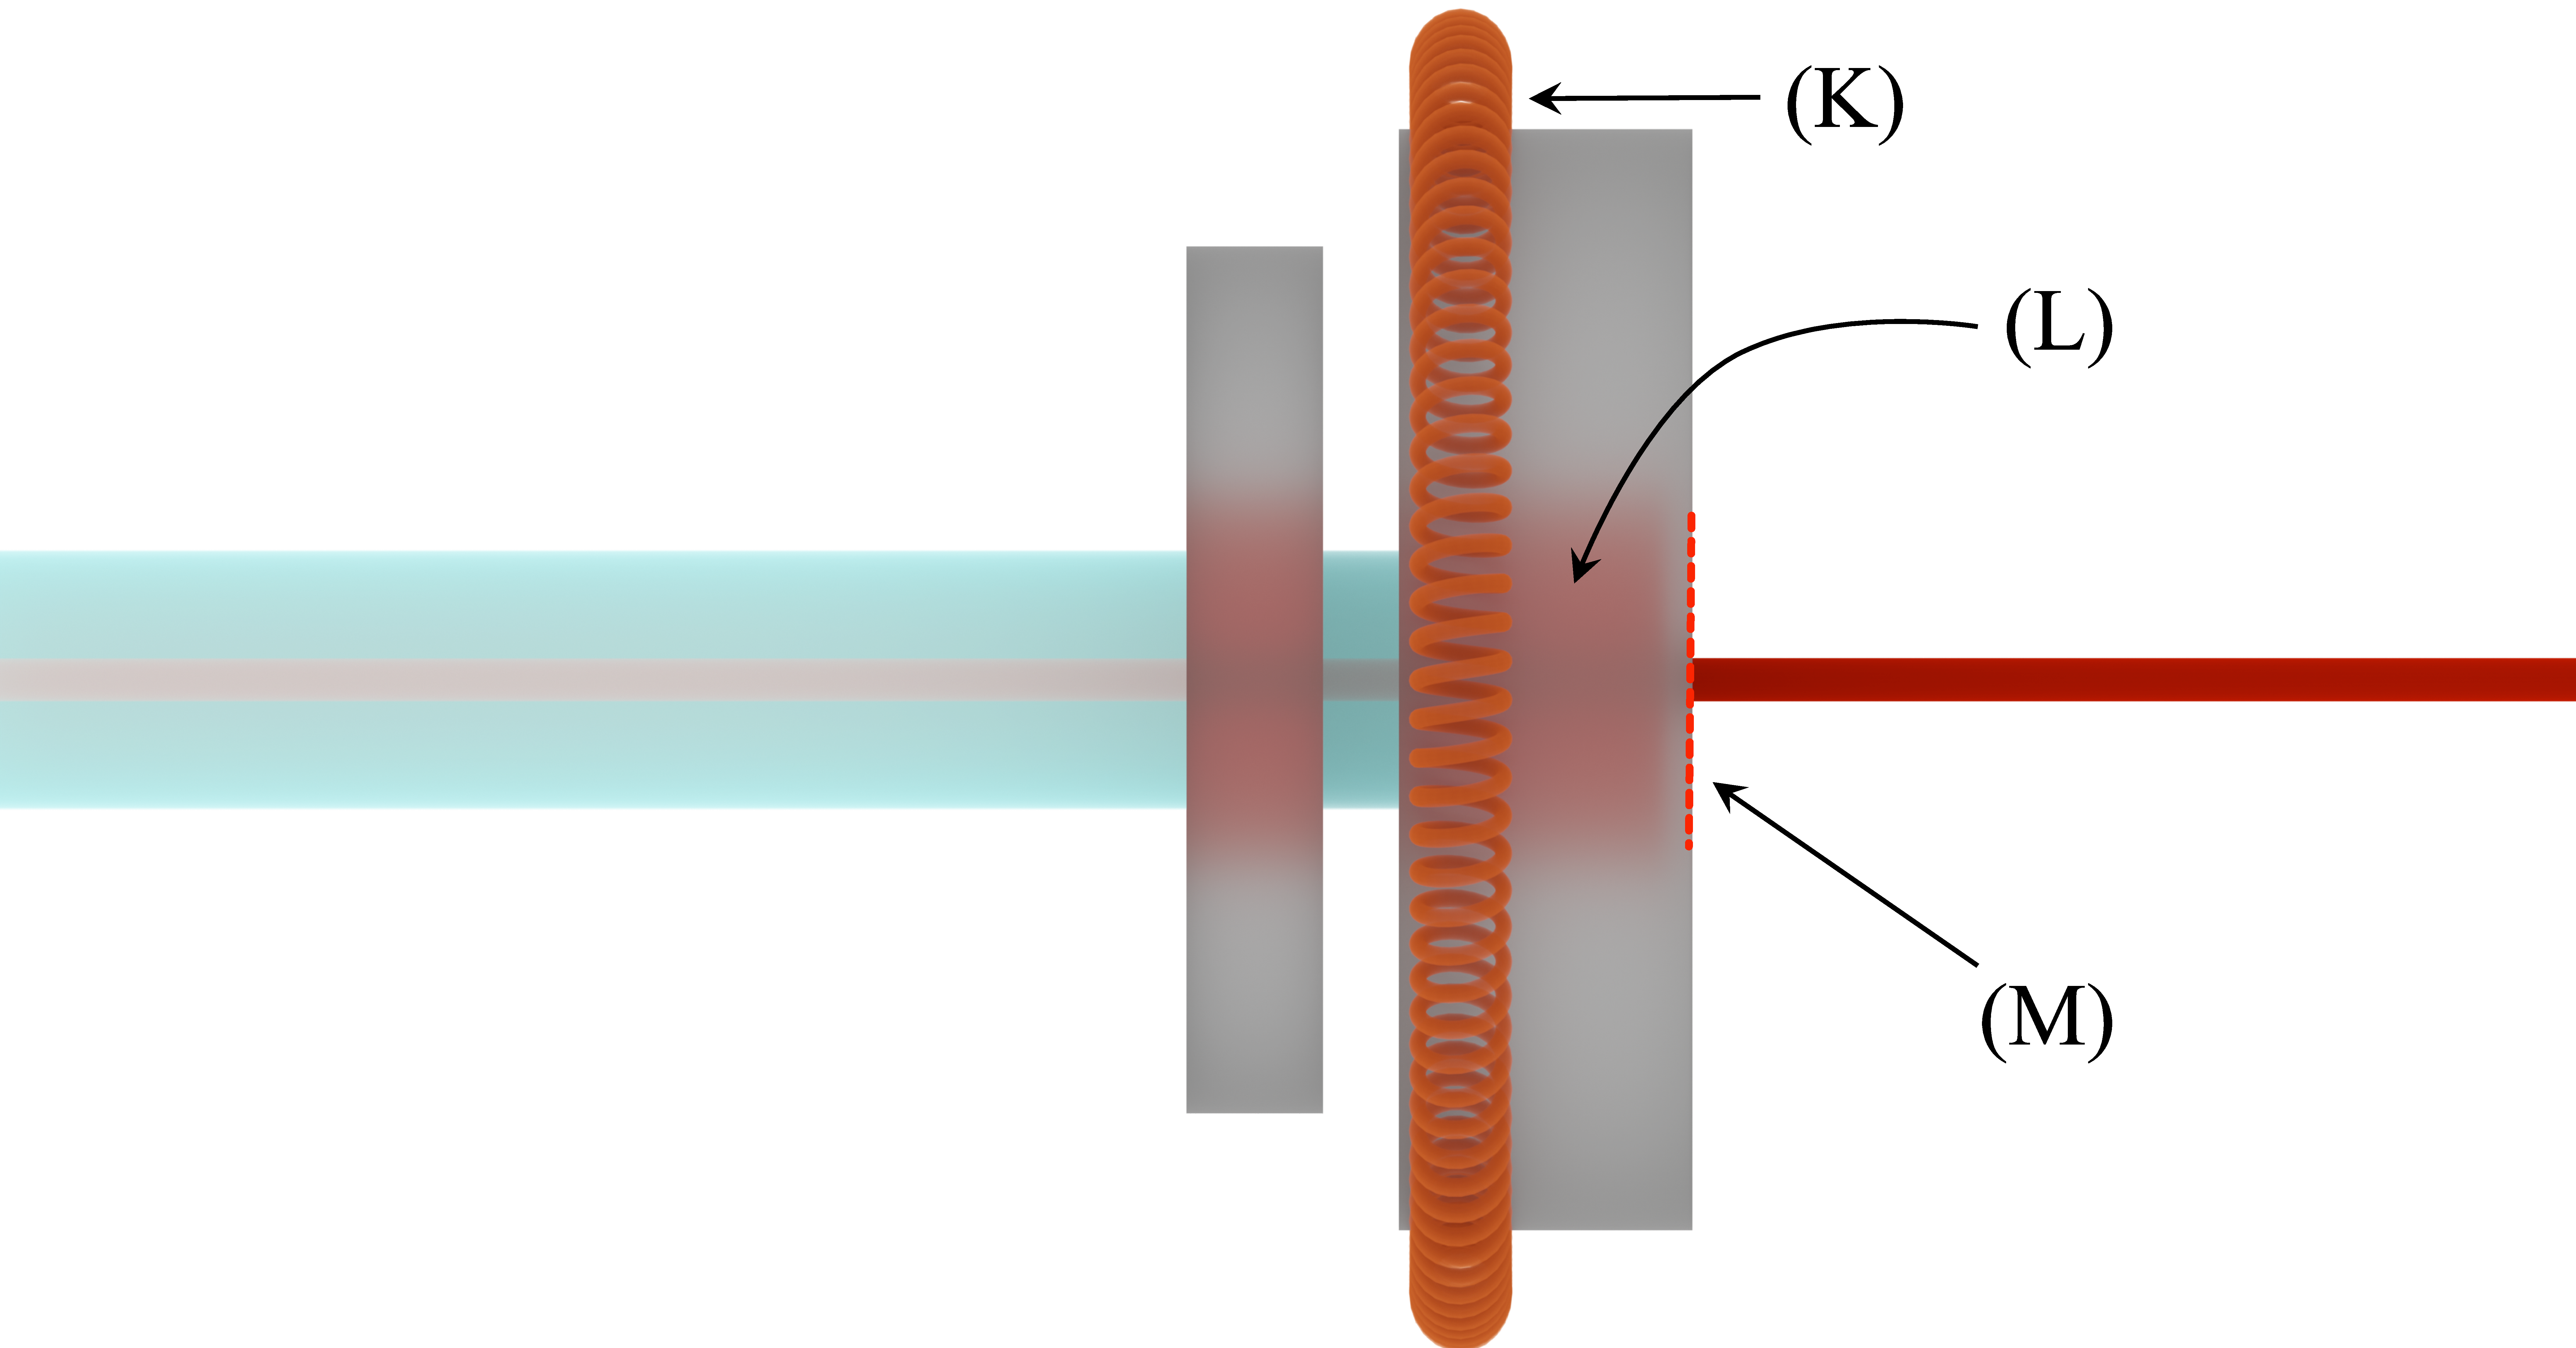
\includegraphics[width=.6\textwidth]{TCS/ITMYarminp/annotated/max/ITMYinp_highcirc.pdf}
		\caption{Maximum circulating arm power, with annular heating and no central CO2 actuation. The careful timing and calibration of the CO2 / RH actuators allow designed power / GW detector sensitivity to be reached.}\label{subfig:TCSinp_highcirc}
%		\caption{Maximum circulating arm power, with annular heating and no central CO2 actuation. The careful timing and calibration of the CO2 / RH actuators allow designed power / GW detector sensitivity to be reached.}\label{TCSinp_highcirc}
	\end{subcaptiongroup}
	\caption{ALIGO thermal compensation design at the input of a single Fabry-P\'{e}rot arm cavity. Though not the only location of thermal mode matching actuators, a careful look here can adequately demonstrates their capabilities and motivates careful tuning while comissioning the current generation of gravitational wave detectors at high power.}
	\label{fig:TCSinp}
\end{figure}

\section{Dynamic Thermal Compensation}
\subsection{Ring heater / test mass thermo-optic response}
Transient ring heater actuation from a radially symmetric thermal aberration ($\Psi(t,r)$) is realized ~\cite{ramette:2016}:

\begin{equation}
	\Psi(t,r)=2\frac{dn}{dT} \sum^{\infty}_{m,p = 1} A_{m,p} \; c^{u}_{p} \mathrm{sin}(u_m h /2a) (a/u_m)[1-e^{-\alpha t}] J_0(\zeta_p r/a)
\end{equation}

\begin{figure}[H]
     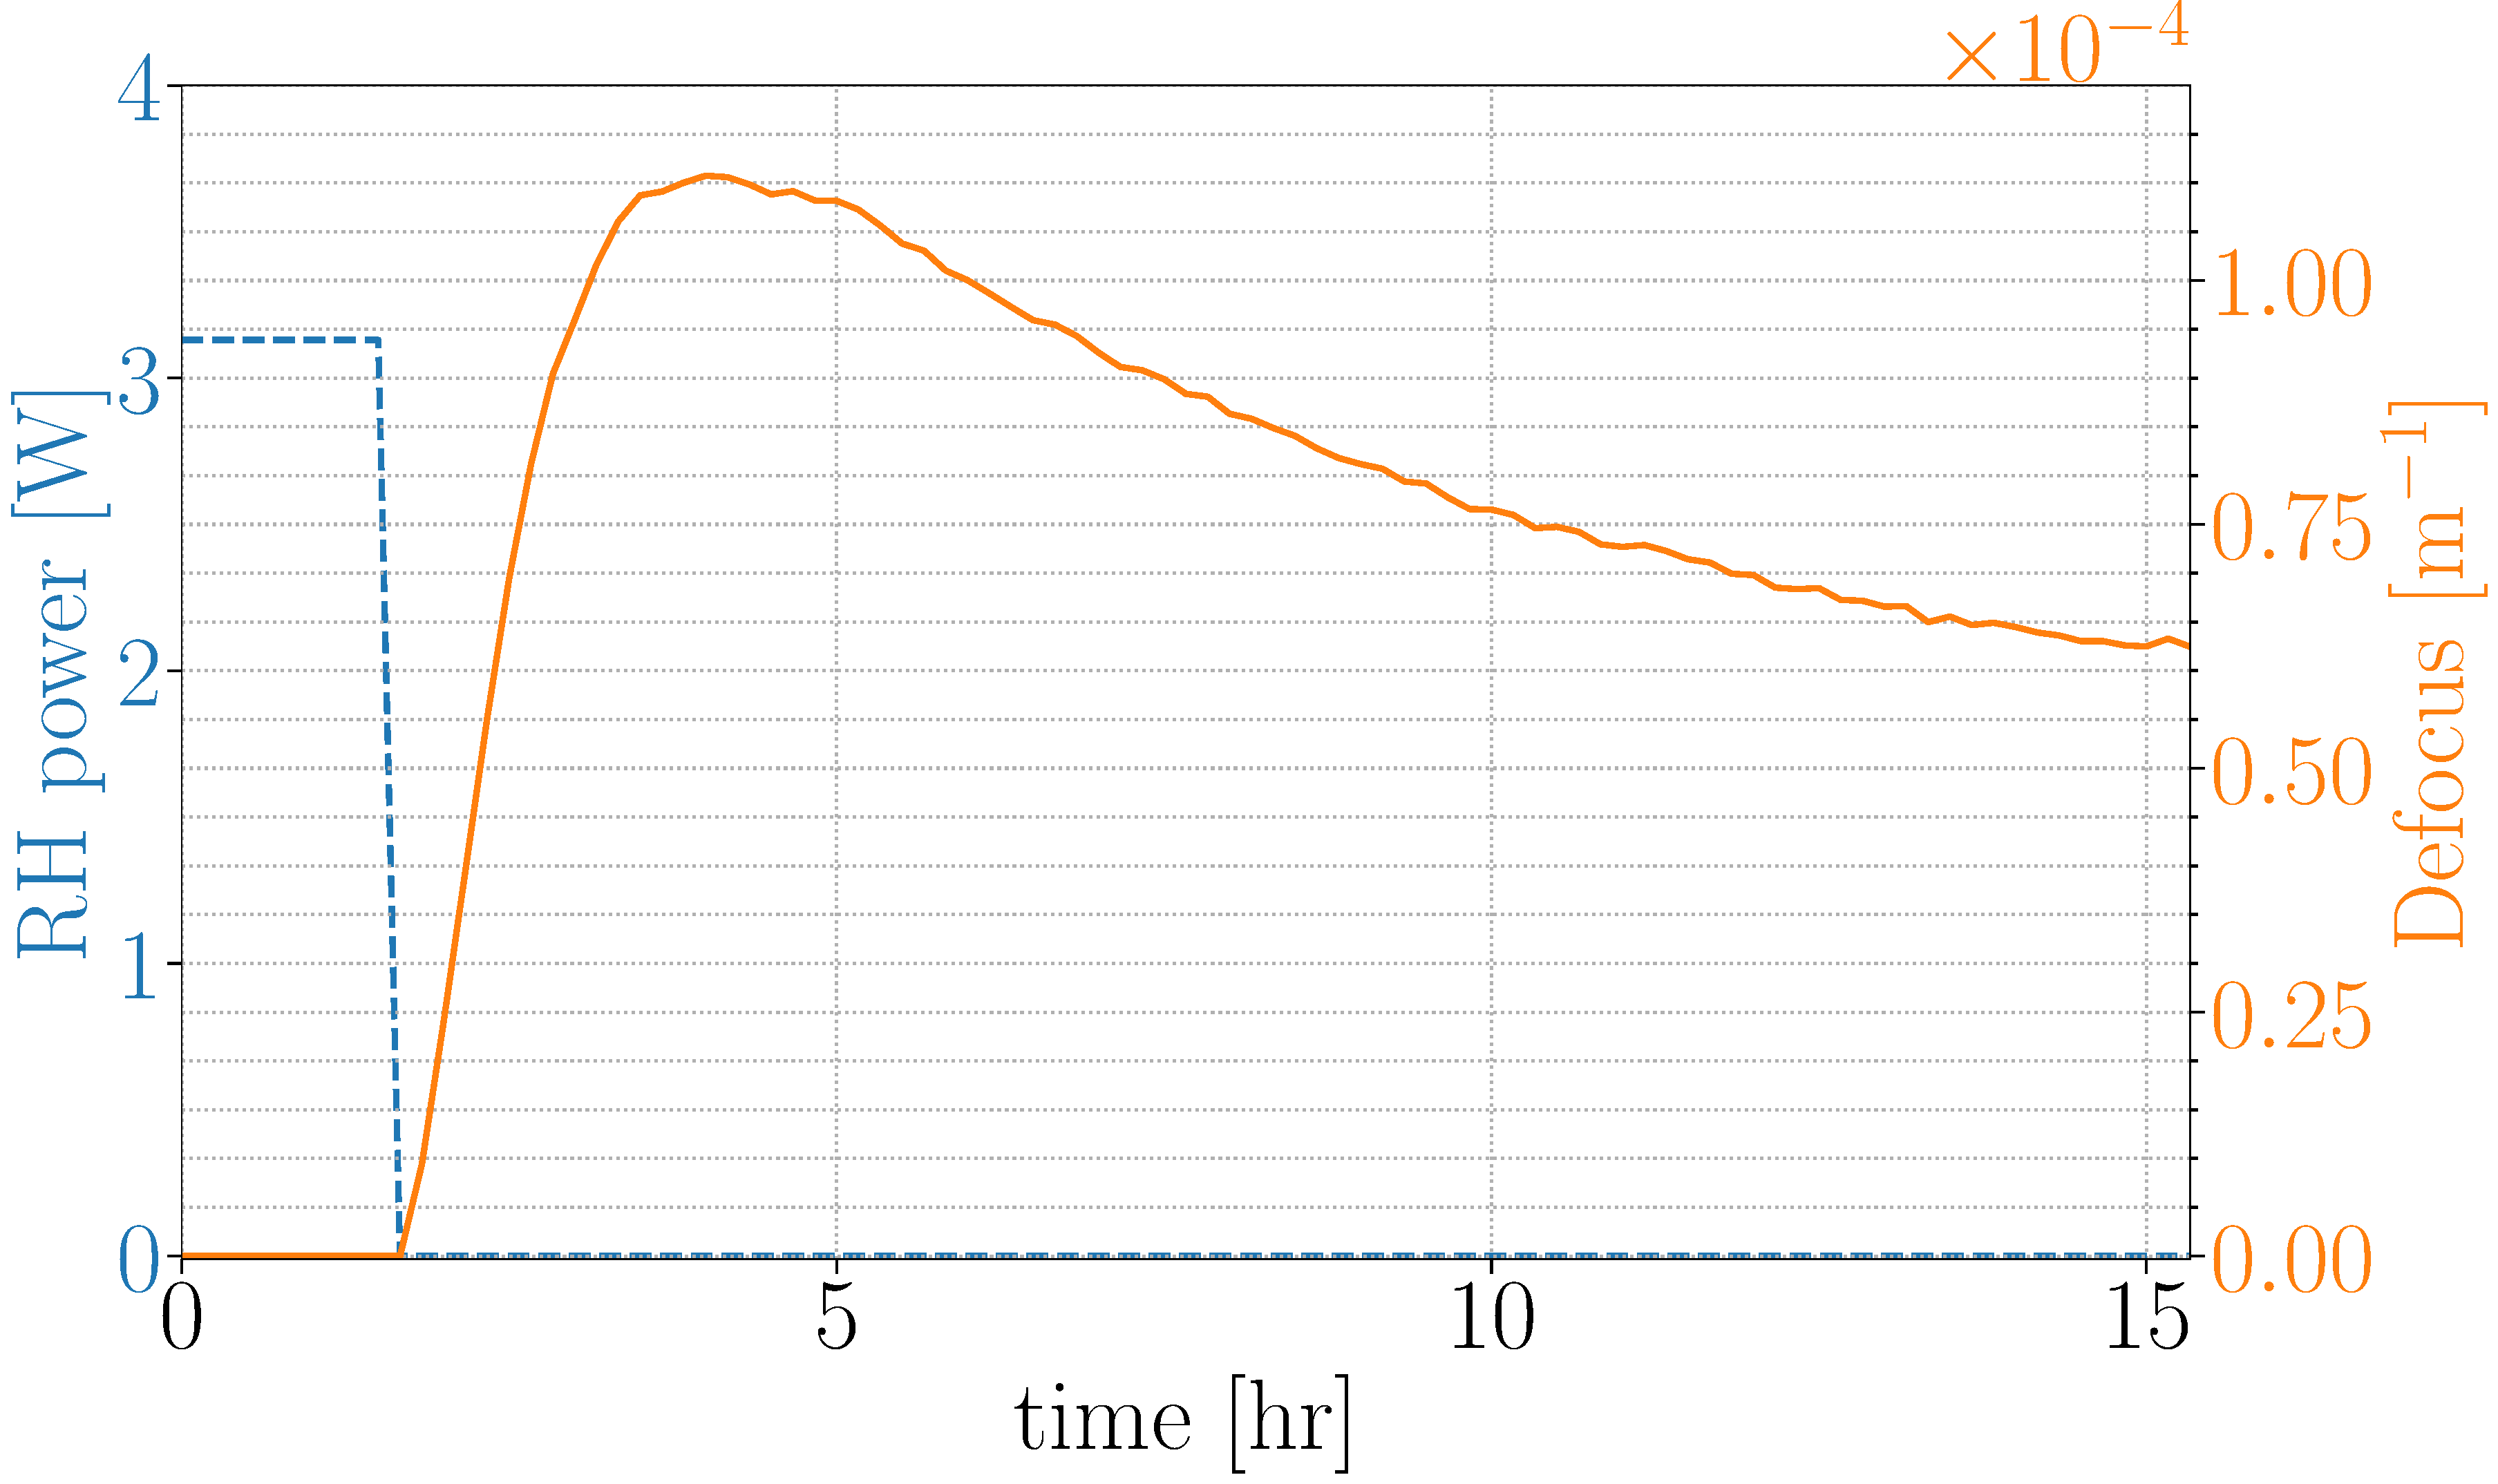
\includegraphics[width=\textwidth]{TCS/IRHF/Meas_response}
     \caption{ITMY thermo-optic response to a 3.13 [W] combined power reduction to the top and bottom ring heater elements. It's after $\approx$ 12 hours after the ring heater power control step do you start to see a small enough steady state differential defocus ($\frac{\mathrm{d} \alpha_\mathrm{sp}}{\mathrm{dt}}$) and can assume a steady state thermal lens. \textcolor{red}{Adding dotted line comparing analytical $\Psi(t,r)$ to measurement.} }
     \label{fig:RHresp}
\end{figure}

The measured thermo-optic step response exhibits differential defocusing for $\approx$ 12 to 15 hours once the ring heater power has been changed; and with a large enough power steps, these adjustments to ring heater power can significantly stall precious detector observing/comissioning time due to differential mode matching. Thermo-optic time constants can be reduced by applying real time digital filtering to ring heater power controls. The desired thermo-optic response is one that resembles a step from one defocus state to another with no intermediate overshoot. 

\begin{figure}[H]
	\centering
	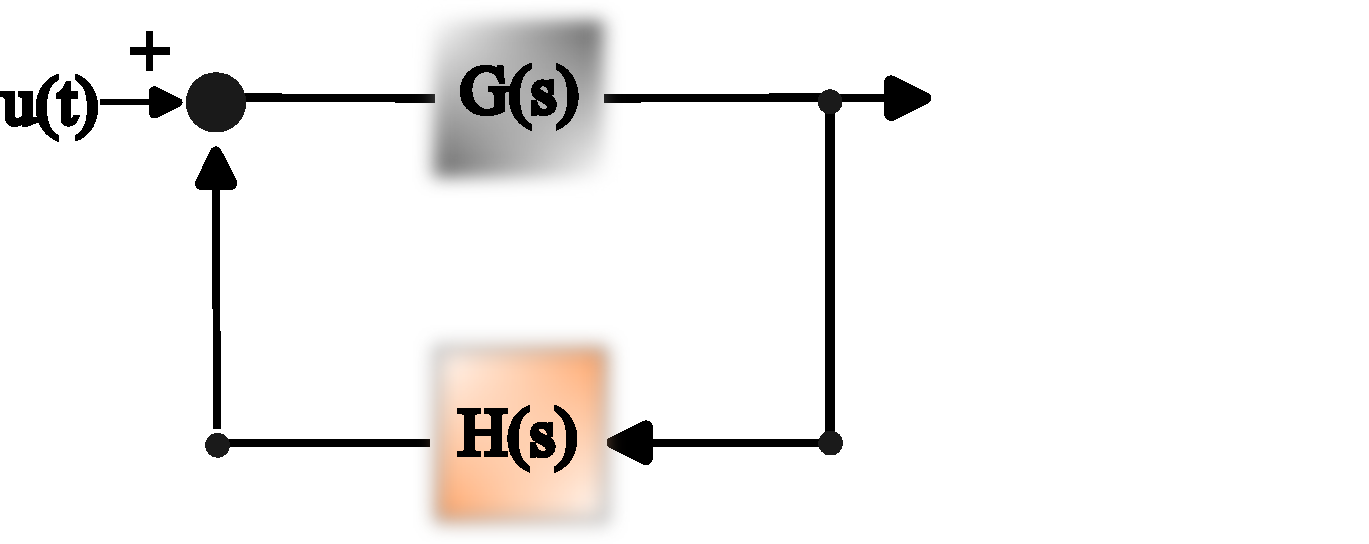
\includegraphics[width=\textwidth]{TCS/IRHF/RH_control_diagram.pdf}
	\caption{Comparison of the natural RH response and the response to the conditioned input. The above plot is simulated in Matlab by passing the RH input time series (top plot) through the $[H(s)]^{-1*}$ and $H(s)$ to acquire with the result lensing behavior on the bottom plot.}
	\label{fig:RH_control}
\end{figure}

\begin{figure}[H]
    \centering
    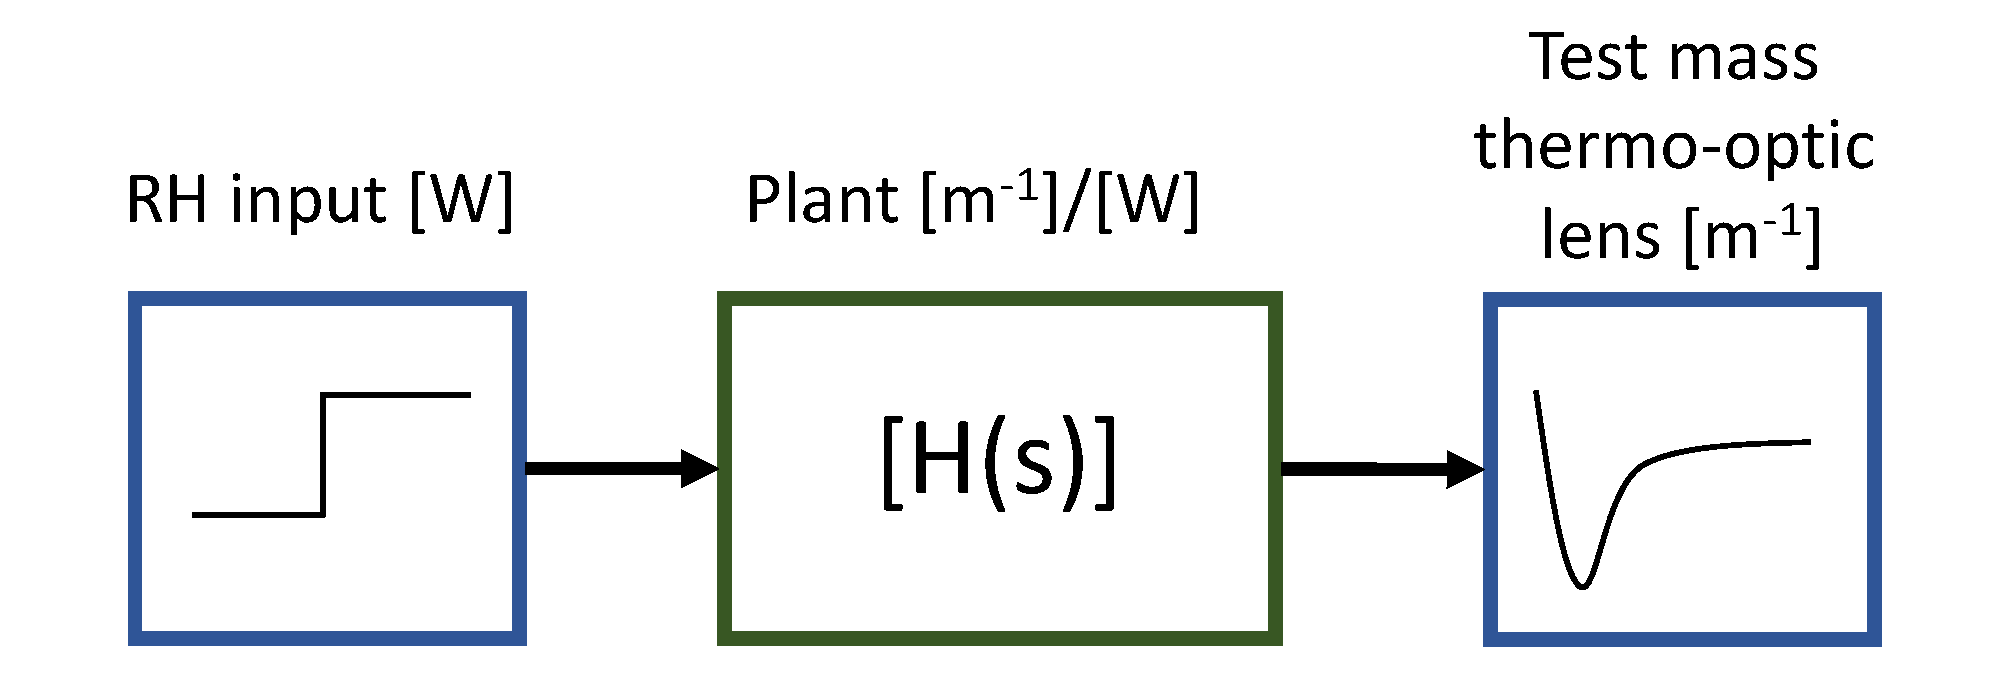
\includegraphics[page=1,width=.75\textwidth]{TCS/IRHF/RH_input_filter_figures.pdf}
    \caption{A feedback-style block pictograph of the plant system (test mass mirror and annular ring heater) transforming the ring heater power control step to a time-varying thermo-optic response. The example of this can be seen in Fig [\ref{fig:RHresp}]}
    \label{fig:justplant}
\end{figure}

As the queried RH power resembles that of a step, inverting this step-response can provide a feasible first order filter. Therefore, the prescription for creating such a filter is realized through inversion of the well known RH step response alongside additional low passing at high frequency to avoid any control instability at high frequency. 

\textcolor{red}{see appendix for more detail}
%\begin{enumerate}[label=\arabic*),leftmargin=75pt,nosep]
%	\item Fit step response to a zpk filter $H(s)$ 
%	\item Invert fitted filter ($H(s) \rightarrow H^{-1}(s)$) 
%	\item Apply correction filter $G(s)$ for stability and speed tuning ($H^{-1}(s)*G(s)$)
%\end{enumerate}

\begin{figure}[H]
    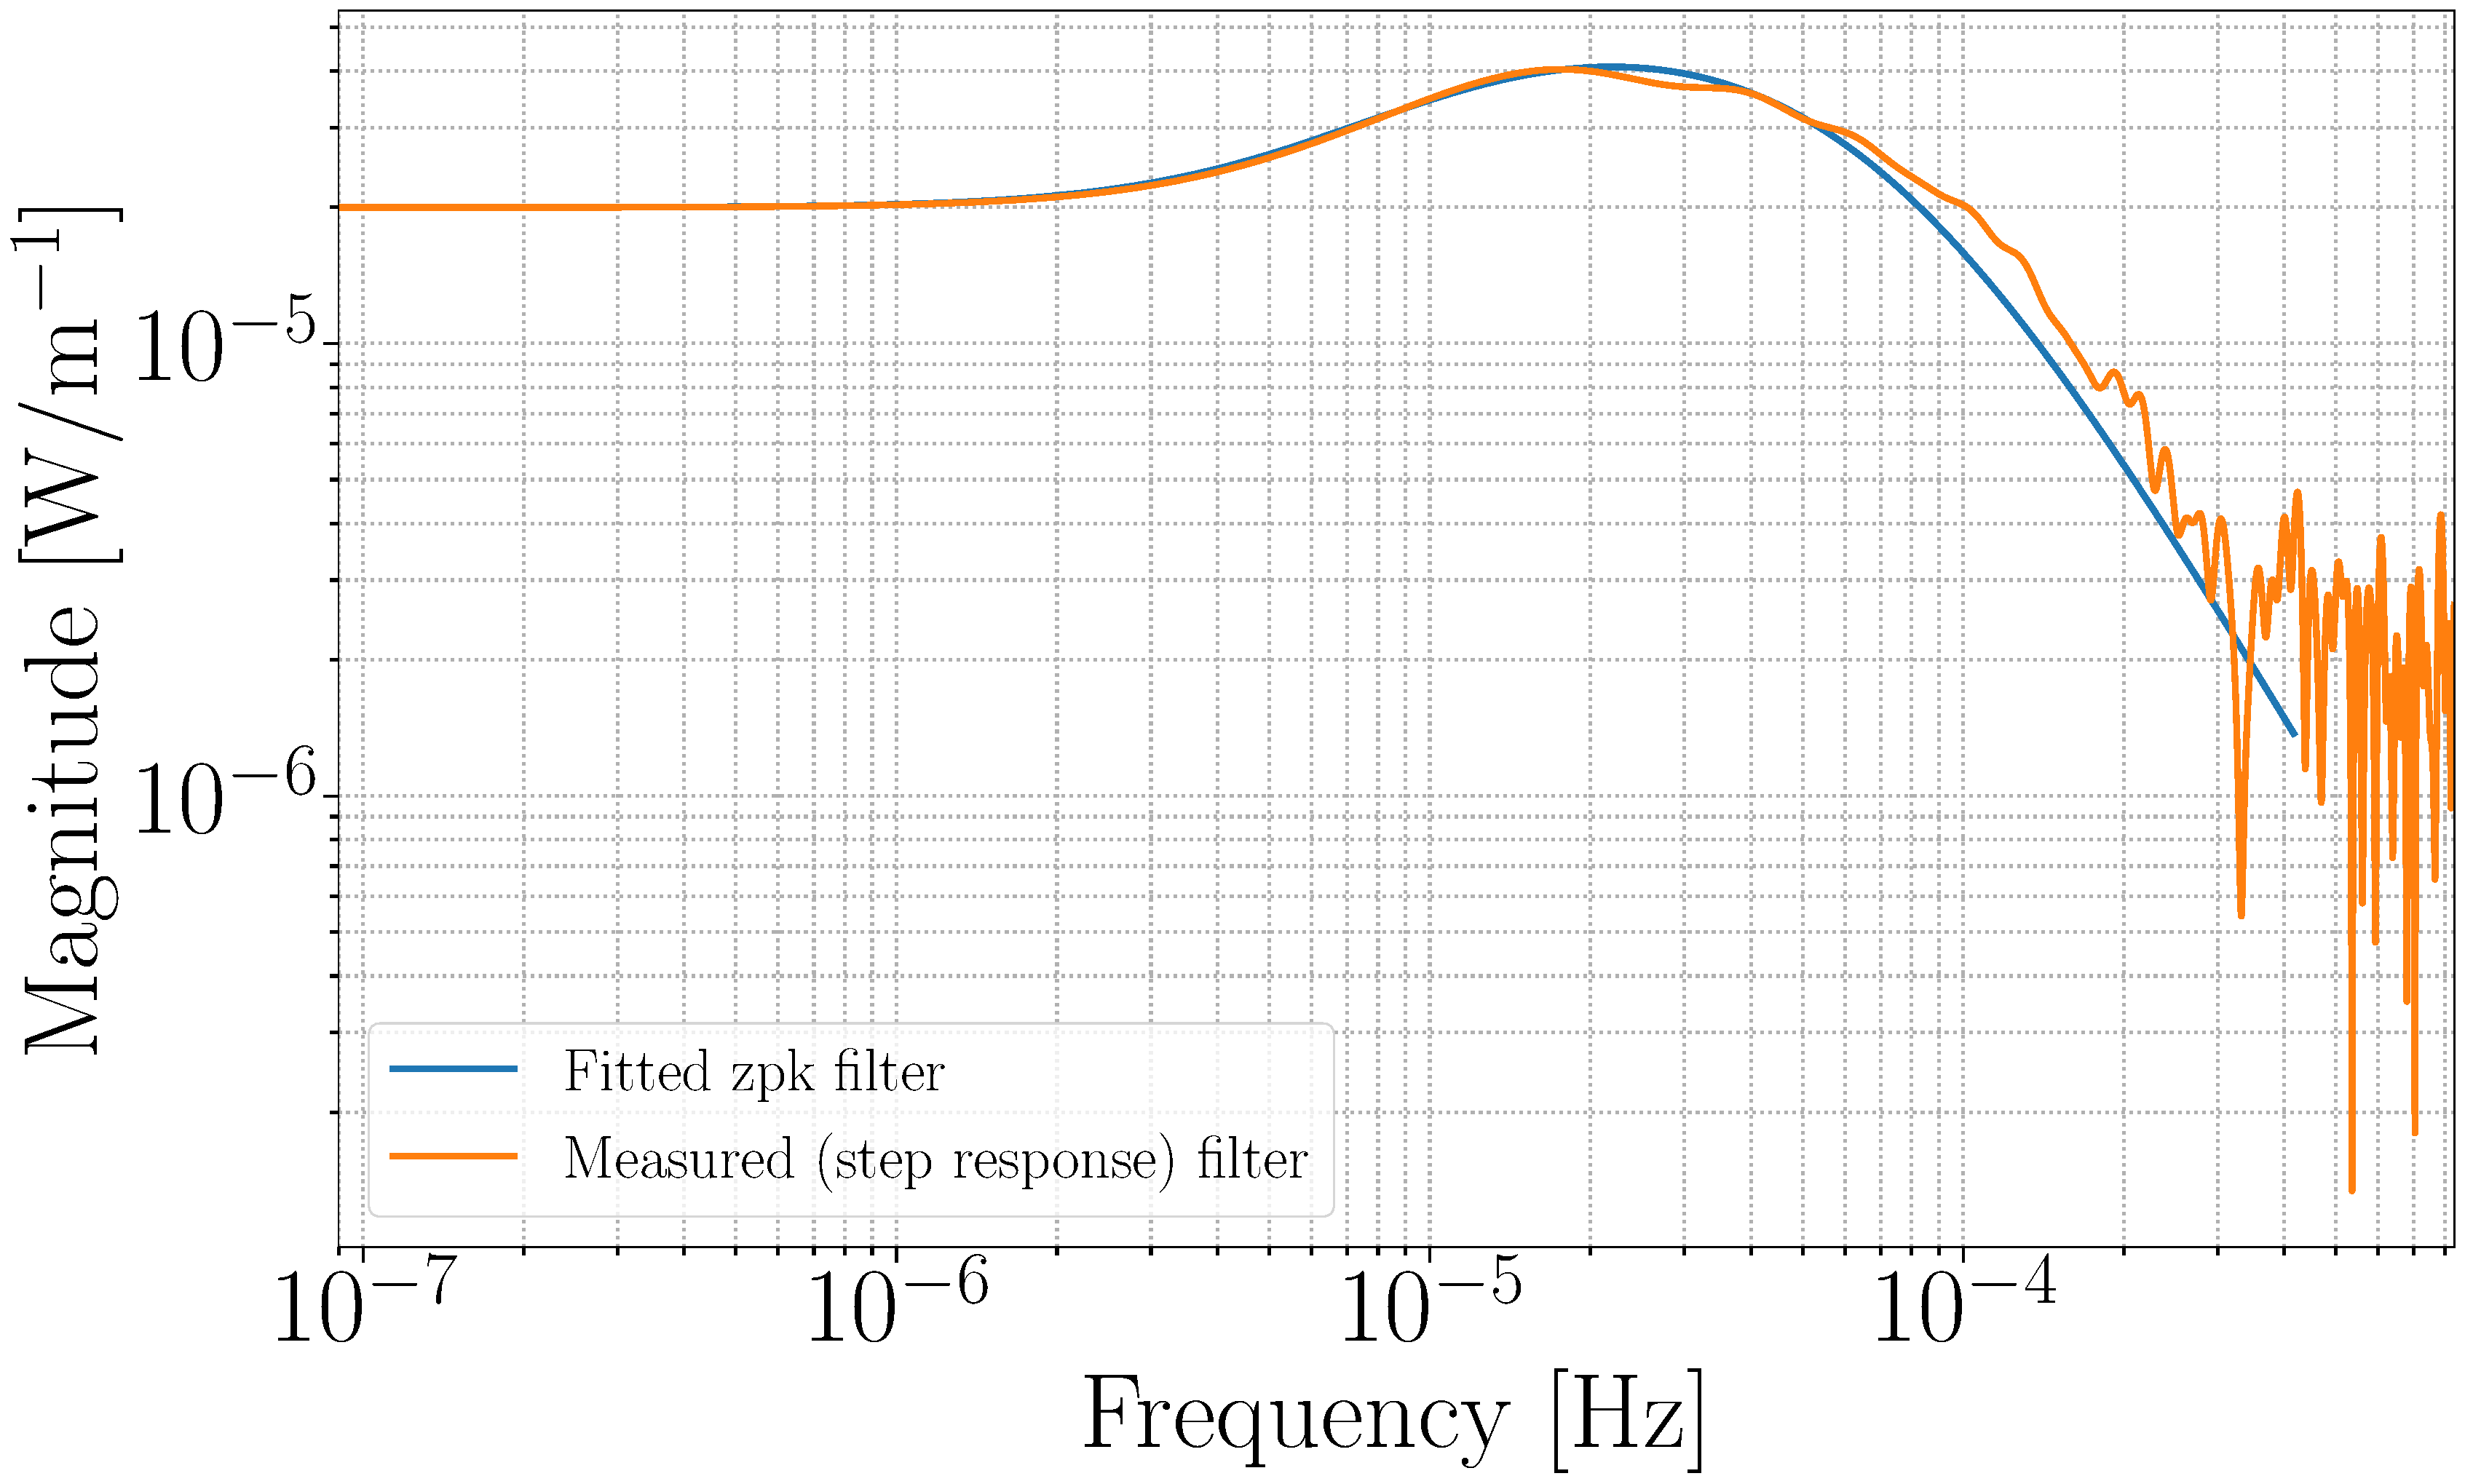
\includegraphics[width=\textwidth]{TCS/IRHF/RH_plant_filter_fit}
    \caption{Showing the PSD of the RH response (normalized by the input RH power) over a an $\approx$ 12.5 hour period. The zpk model of the fitted filter (H(s)) = $9.2545\mathrm{e} \text{-}12 \Big(\frac{(s+3.14210\mathrm{e}\text{-}5)}{(s+8.168\mathrm{e}\text{-}5)(s+0.0003142)(s+0.0005969)}\Big)$}
    \label{fig:plant_v_fit}
\end{figure}

\begin{figure}[H]
    \centering
    \includegraphics[page=2,width=.9\textwidth]{TCS/IRHF/RH_input_filter_figures.pdf}
    \caption{A pictograph showing the system with real time digital filtering for an improved thermo-optic response. The RH input filter is created by inverting the plant filter combine with a low pass and added poles to the zpk model to ensure stability.}
    \label{fig:rtdf_pictograph}
\end{figure}

\begin{figure}[H]
    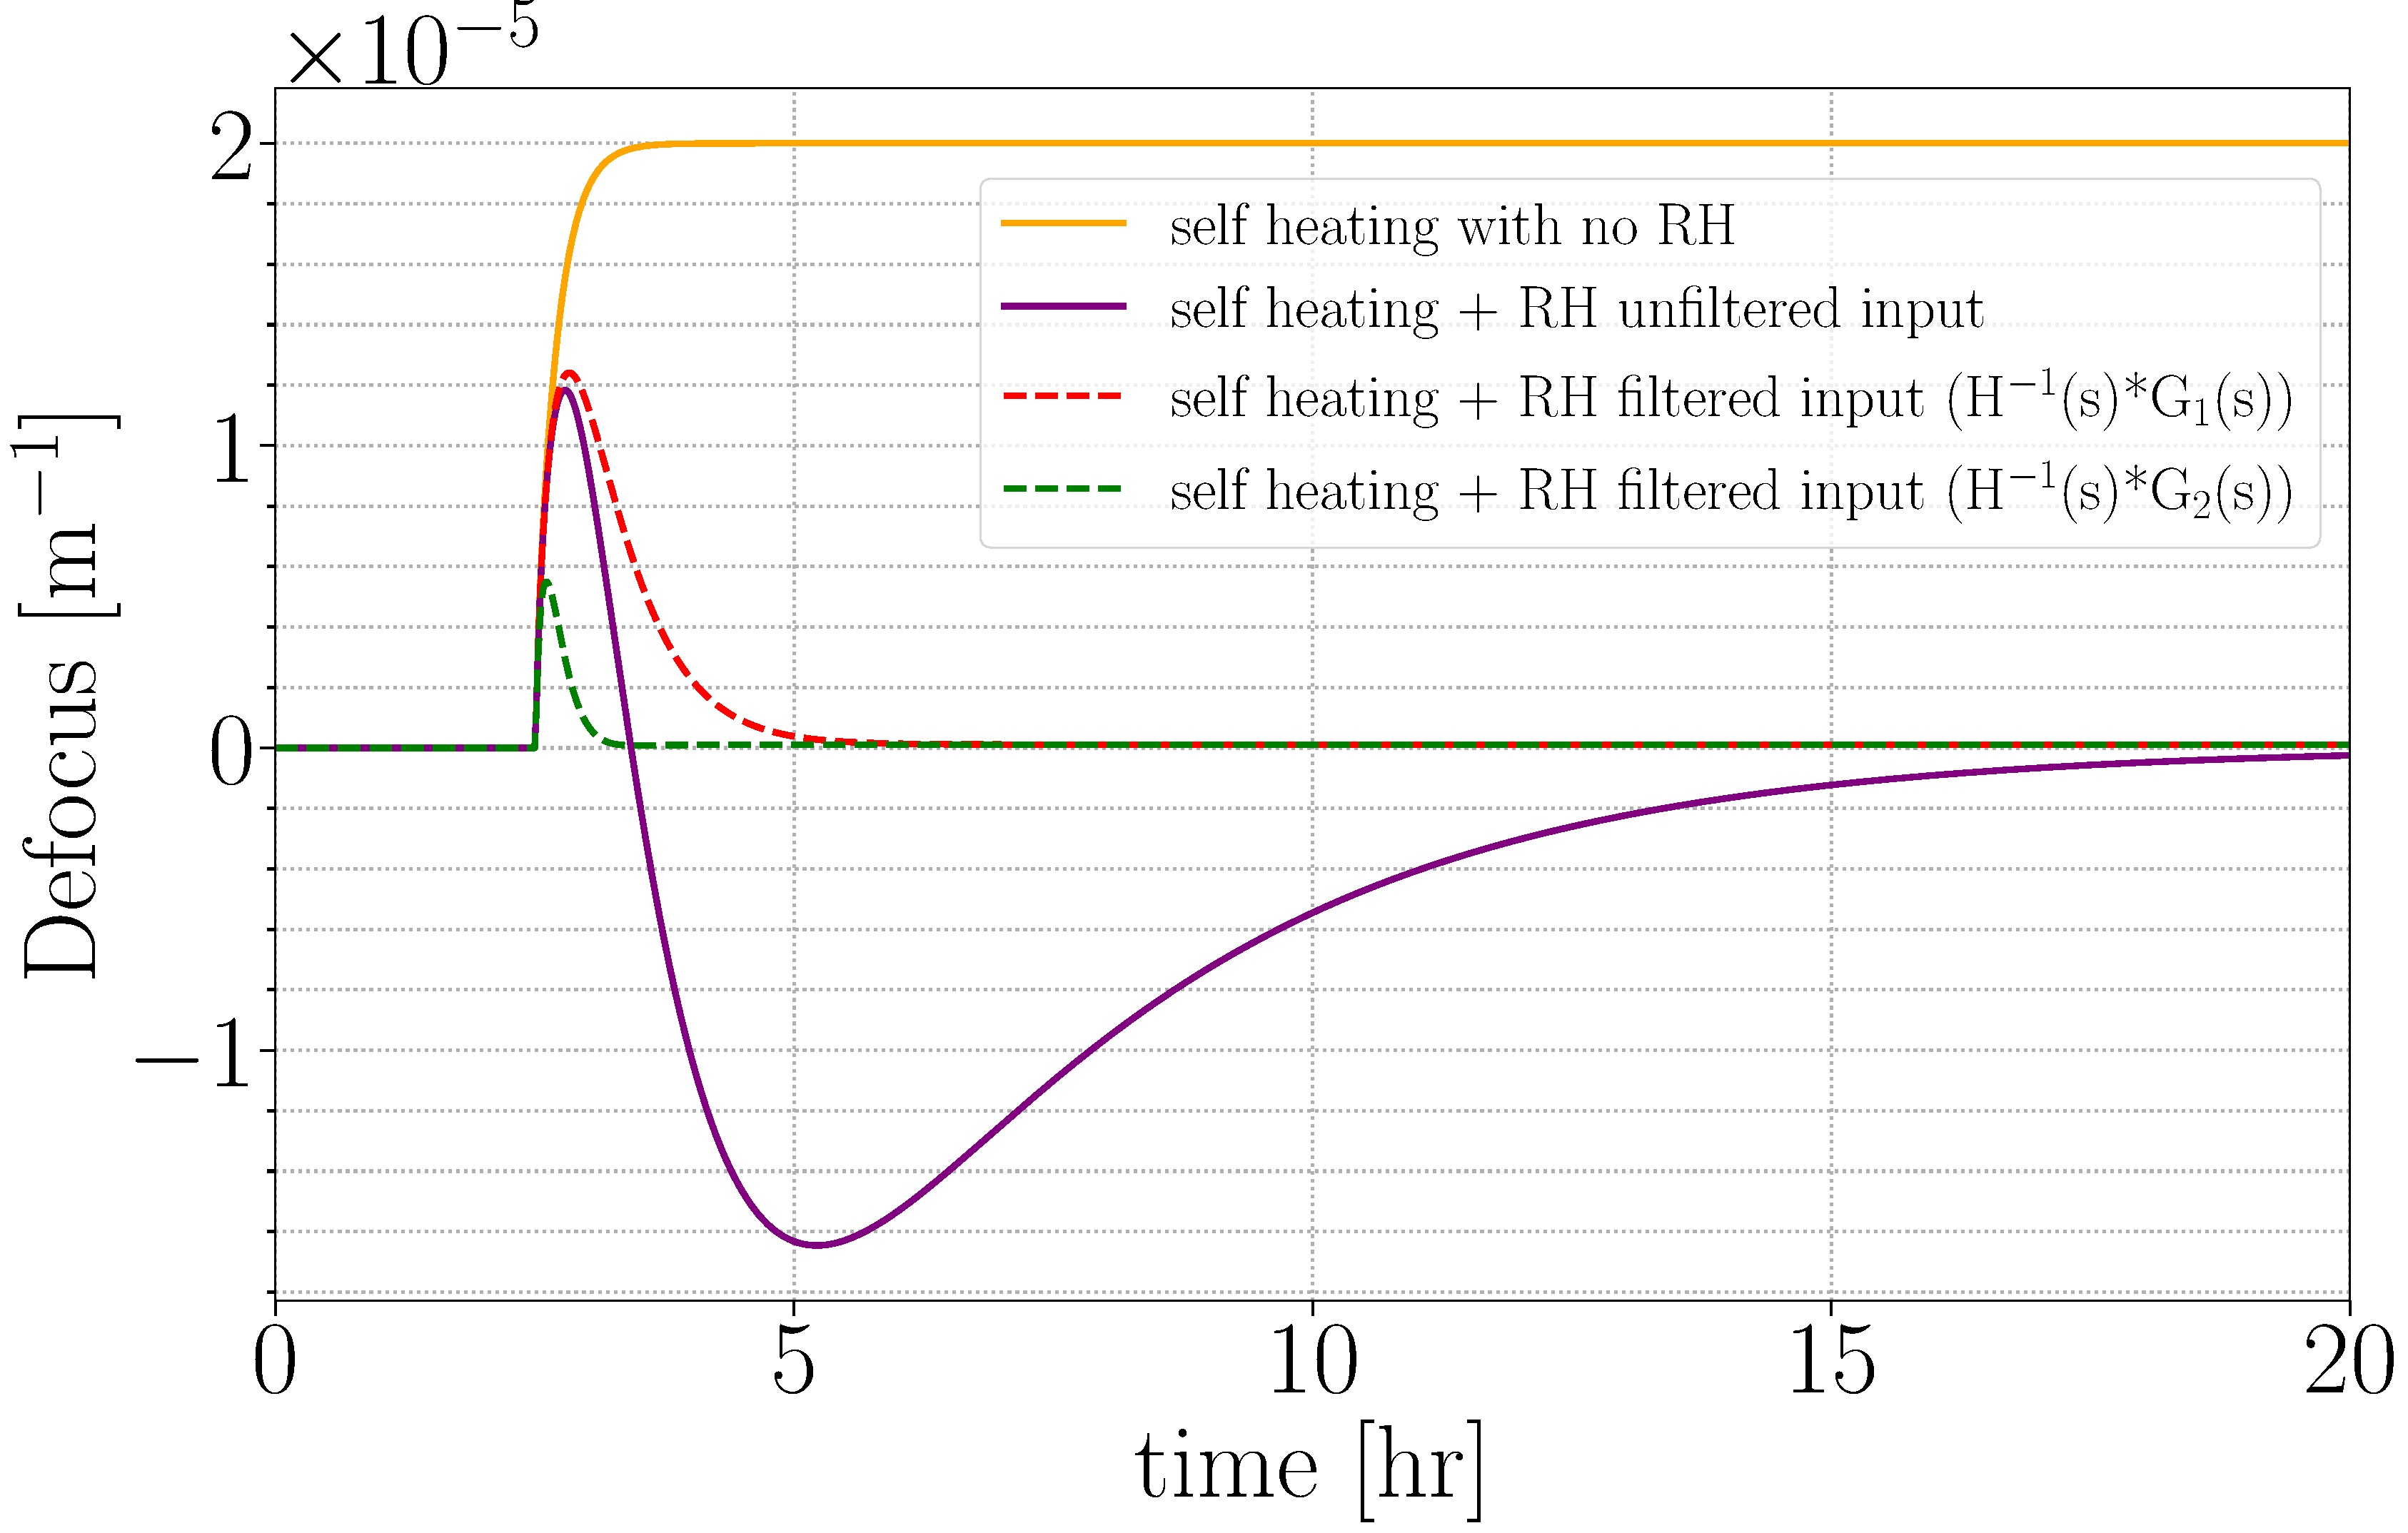
\includegraphics[width=\textwidth]{TCS/IRHF/IRHF_compare_w_self}
    \caption{Comparison of the natural RH response and the response to the conditioned input. The above plot is simulated in Matlab by passing the RH input time series (top plot) through the $[H(s)]^{-1*}$ and $H(s)$ to acquire with the result lensing behavior on the bottom plot.}
    \label{fig:dynam_comparison}
\end{figure}

\subsection{Reducing Parametric Instabilities}
Another symptom of resonant high power optical cavities are parametric instabilities (PI); induced by the opto-mechanical interaction between test mass acoustic modes and higher order optical modes. These PIs present threats to achieving designed detector sensitivity, even driving the detector to lockloss. Passive methods of mitigating PIs by way of acoustic mode dampers (AMD) demonstrate significant reductions of problematic mechanical modes though some (i.e. @ 15 kHz mode) have remained problematic. Lingering parametric instabilities required manual intervention by way of adjusting test mass / cavity geometry to disrupt these persistent PIs, and is now a much more feasible solution with DTC \cite{hardwick:2020}.  

\subsubsection{Limitations}
    \begin{figure}[H]
    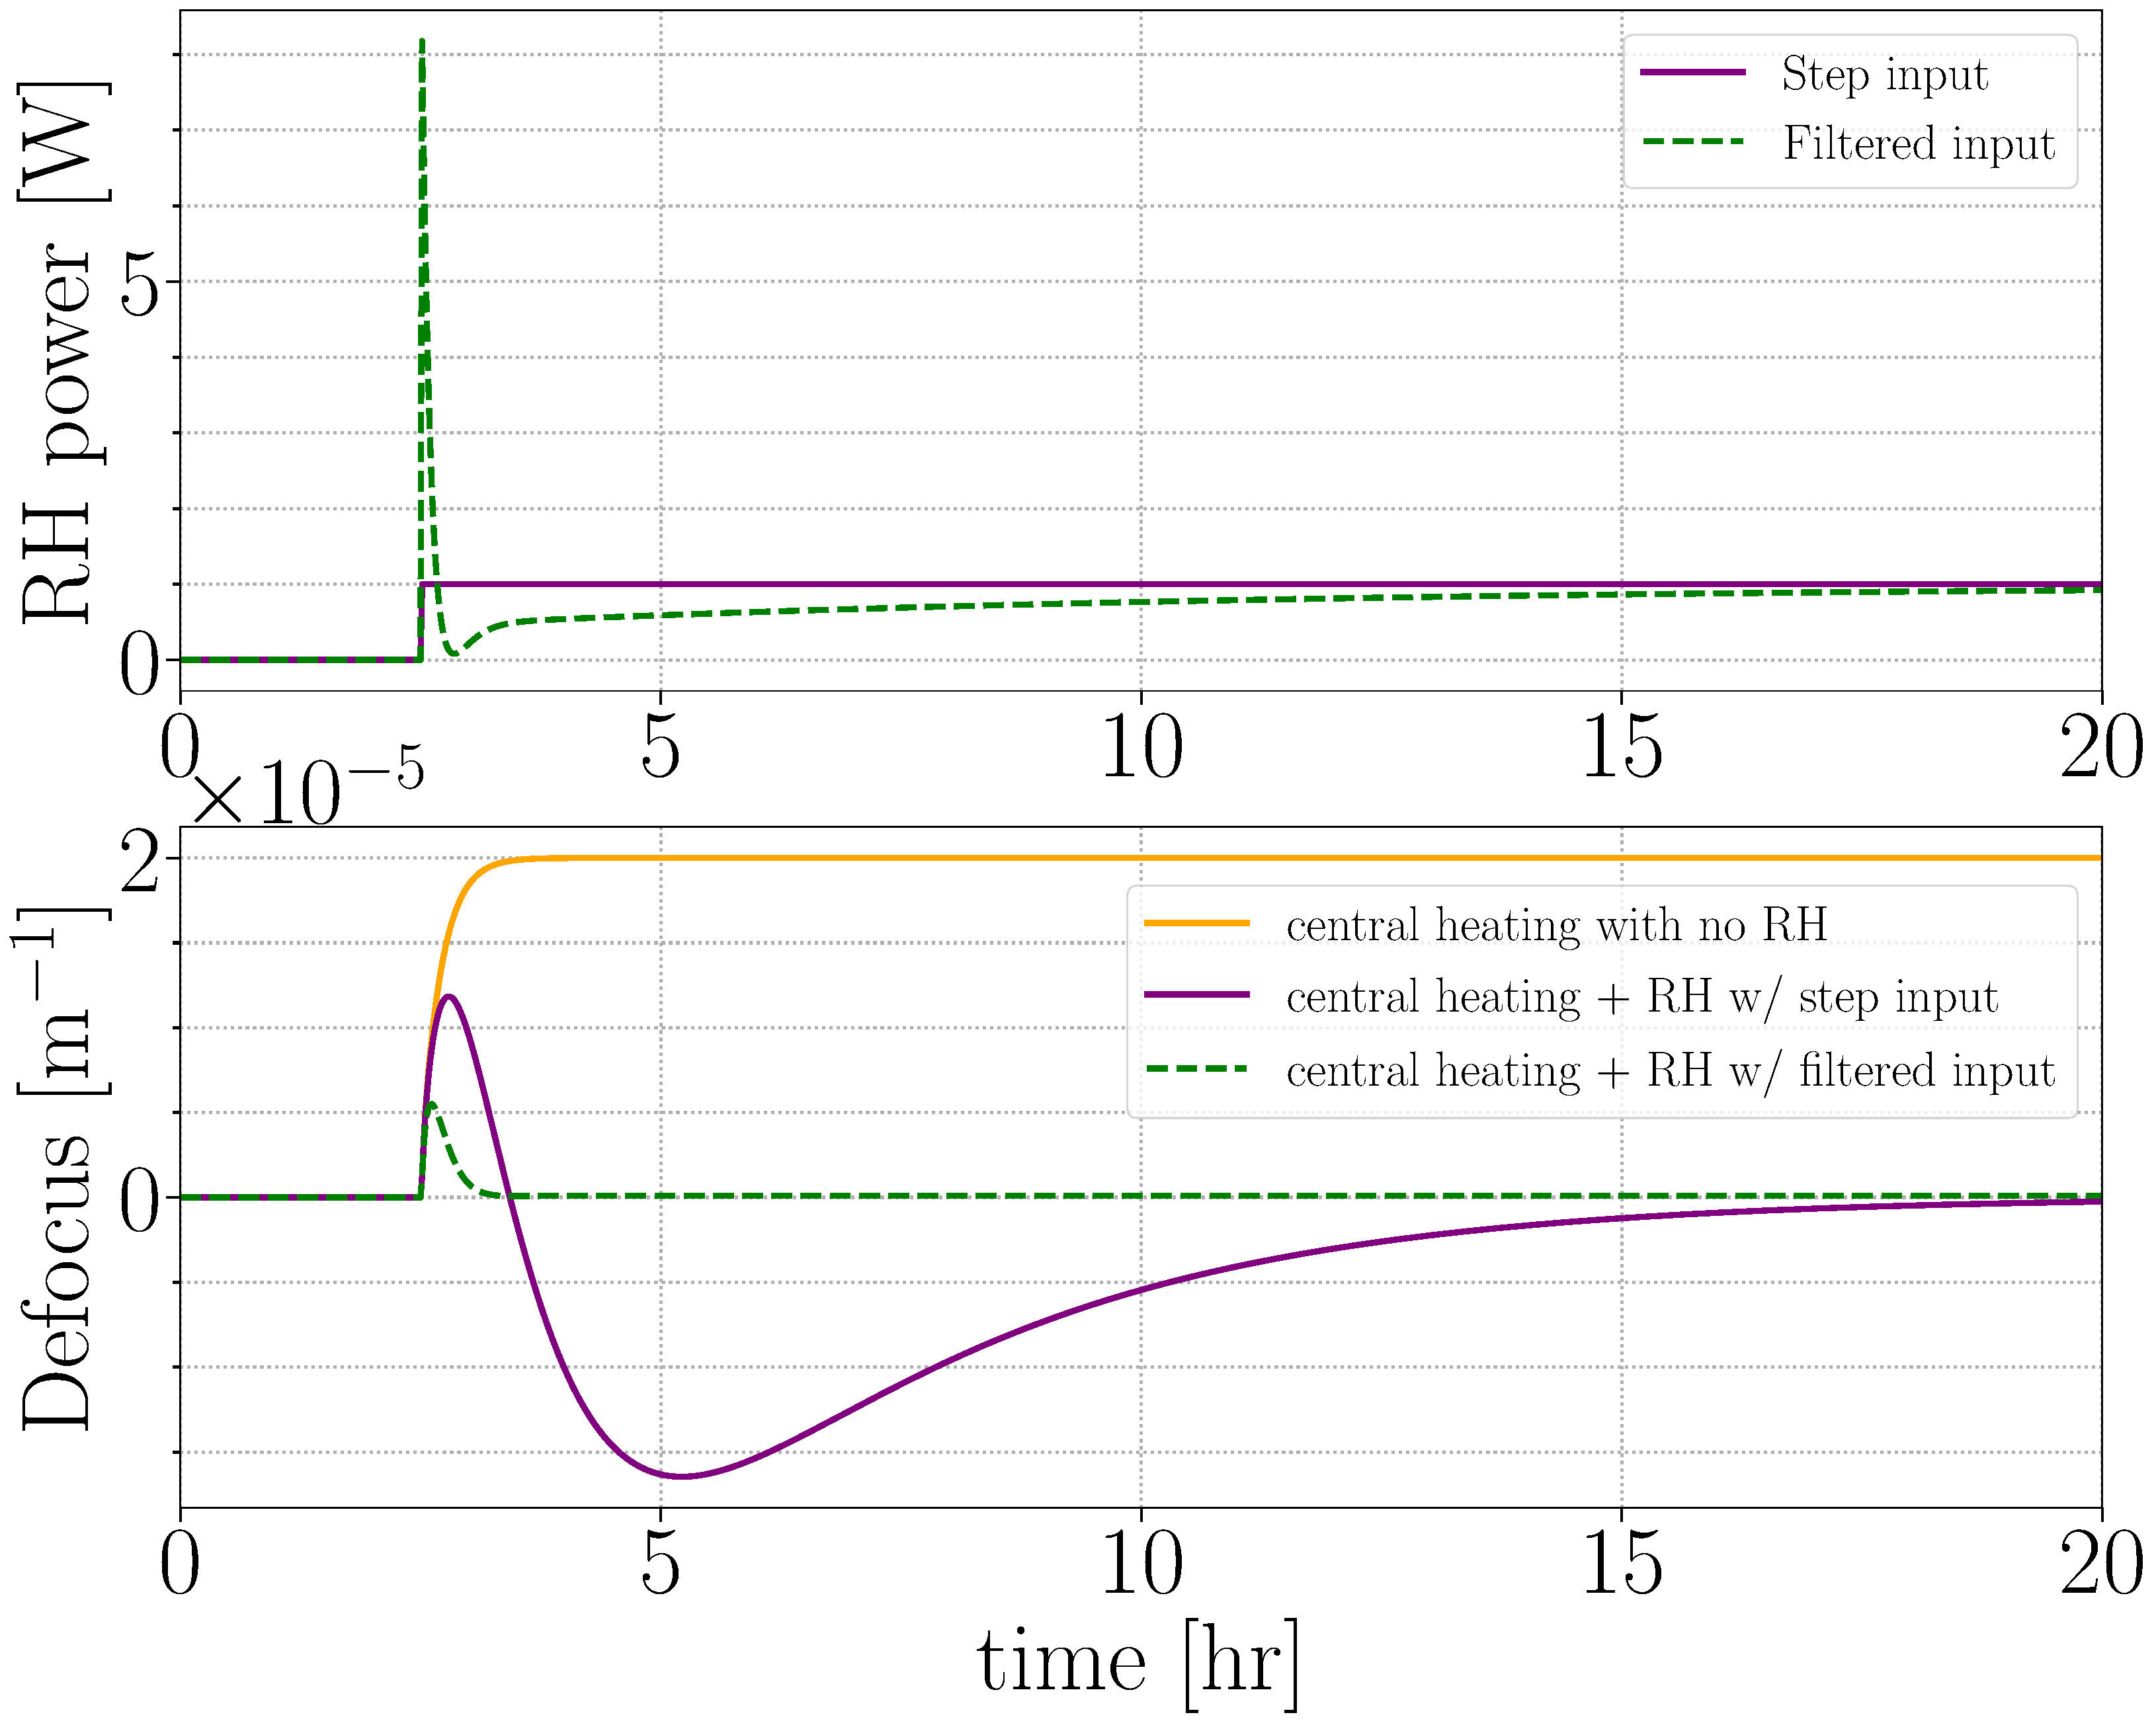
\includegraphics[width=\textwidth]{TCS/IRHF/IRHF_compare_filts_PI_paper}
    \caption{Comparison of the natural RH response and the response to the filtered input with RH power}
    \label{fig:RH_power}
\end{figure}
Limitation on RH power control is set at 10W. \cite{dcc:rhspec}

\section{A priori TCS pre-load methodology for O3a}
Preserving arm cavity resonances requires countering the positive thermal lens defocus of the nominal test mass lens induced by high circulating interferometer arm cavity power. Preparing for this central uniform test mass distortion from the carrier beam requires calibrated and well established thermal actuator settings which in turn informs how much to `pre-load' the TCS actuators using early estimates of test mass absorption. Initial order of magnitude estimates of wavefront distortion from ultra-low absorption fused silica test masses under the influence of a centered high power gaussian beam as well as annular ring heater actuation are available \cite{hellovinet:1990, ramette:2016}; though variations of the absorption between any two test mass mirrors are accounted for through calibrated defocus measurements using the Hartmann wavefront sensors sensitive to auxilary beams imaged onto the test mass mirror surfaces. Measured wavefront distortion can then be mapped in real time to Zernike polynomial coefficients (i.e. $Z^{l \shorteq 0}_{n \shorteq 2}$) to compute a differential defocus in diopters.

\begin{figure}[H]
  \centering
  \begin{subcaptiongroup}
	  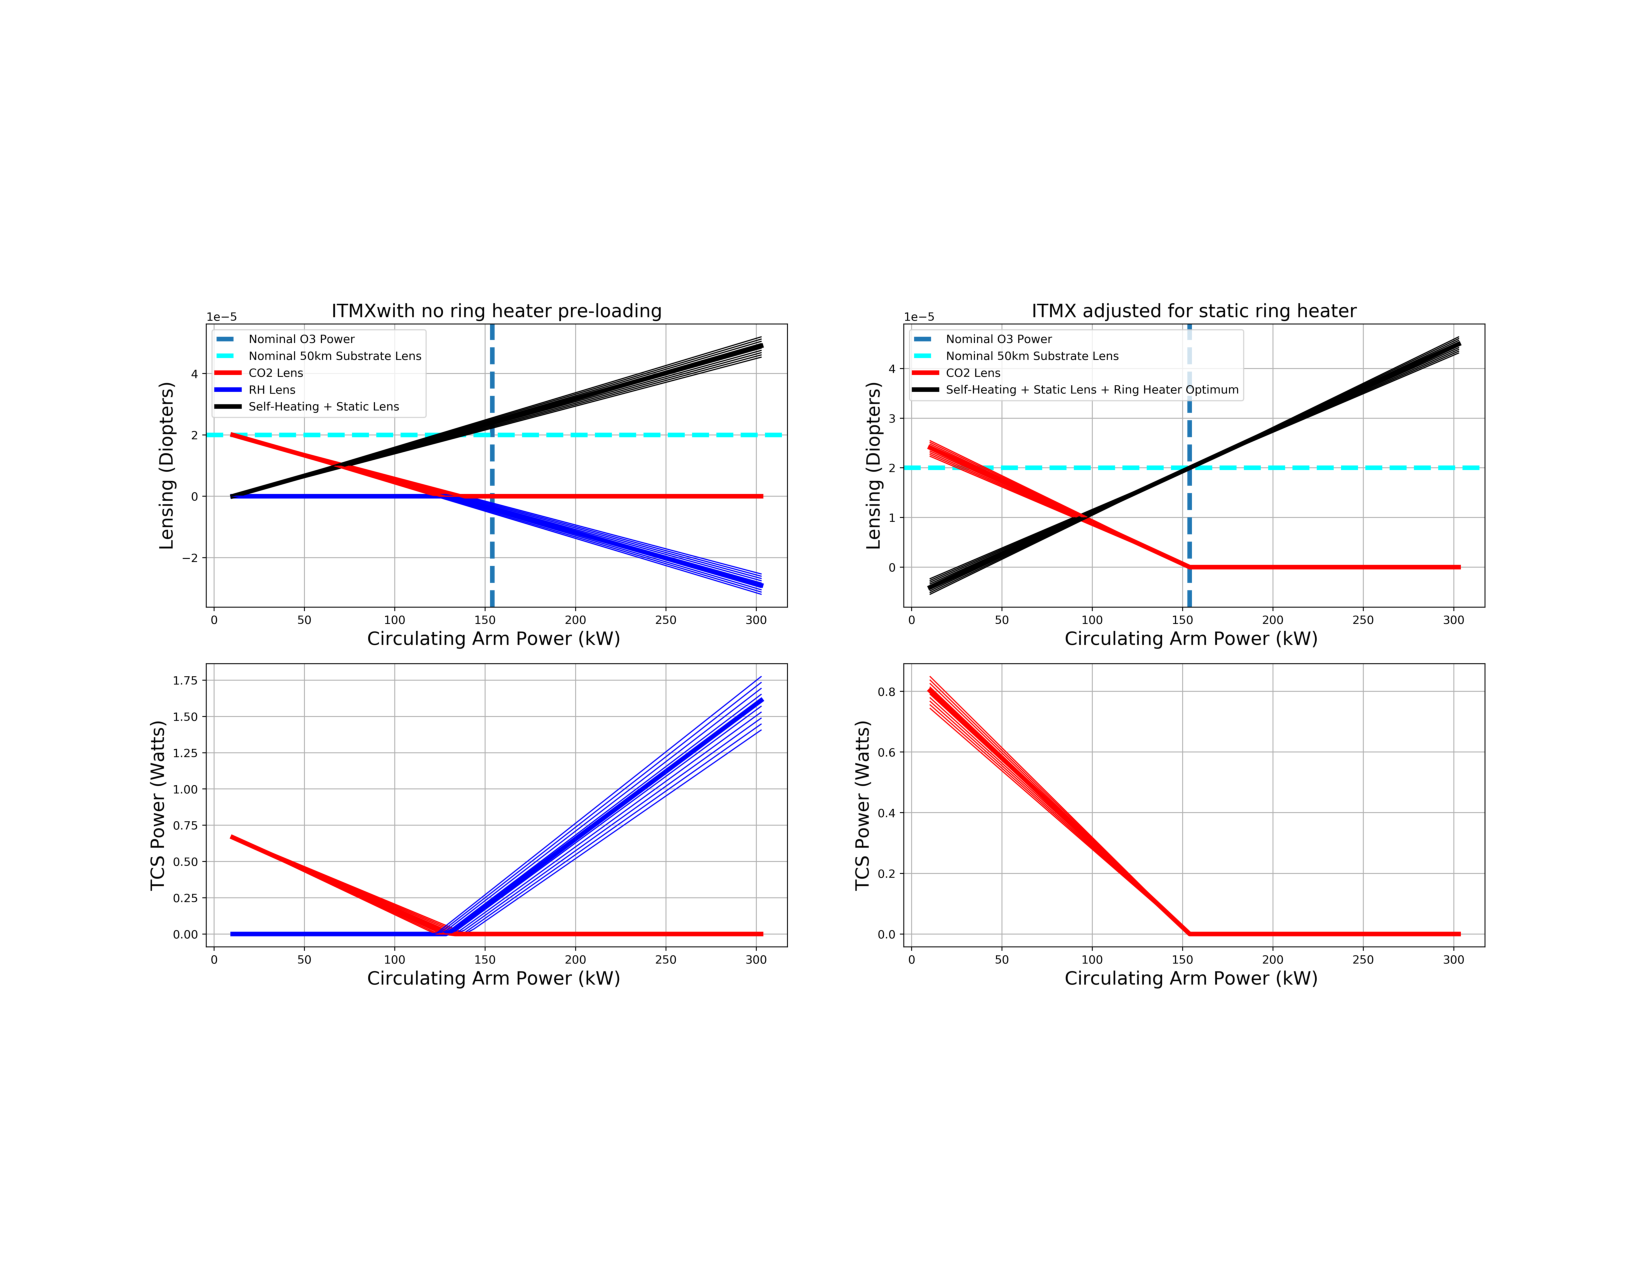
\includegraphics[width=\textwidth]{TCS/ITMX_TCS_Settings_tvo.pdf}
	  \phantomcaption\label{ITMX_TCS}
	  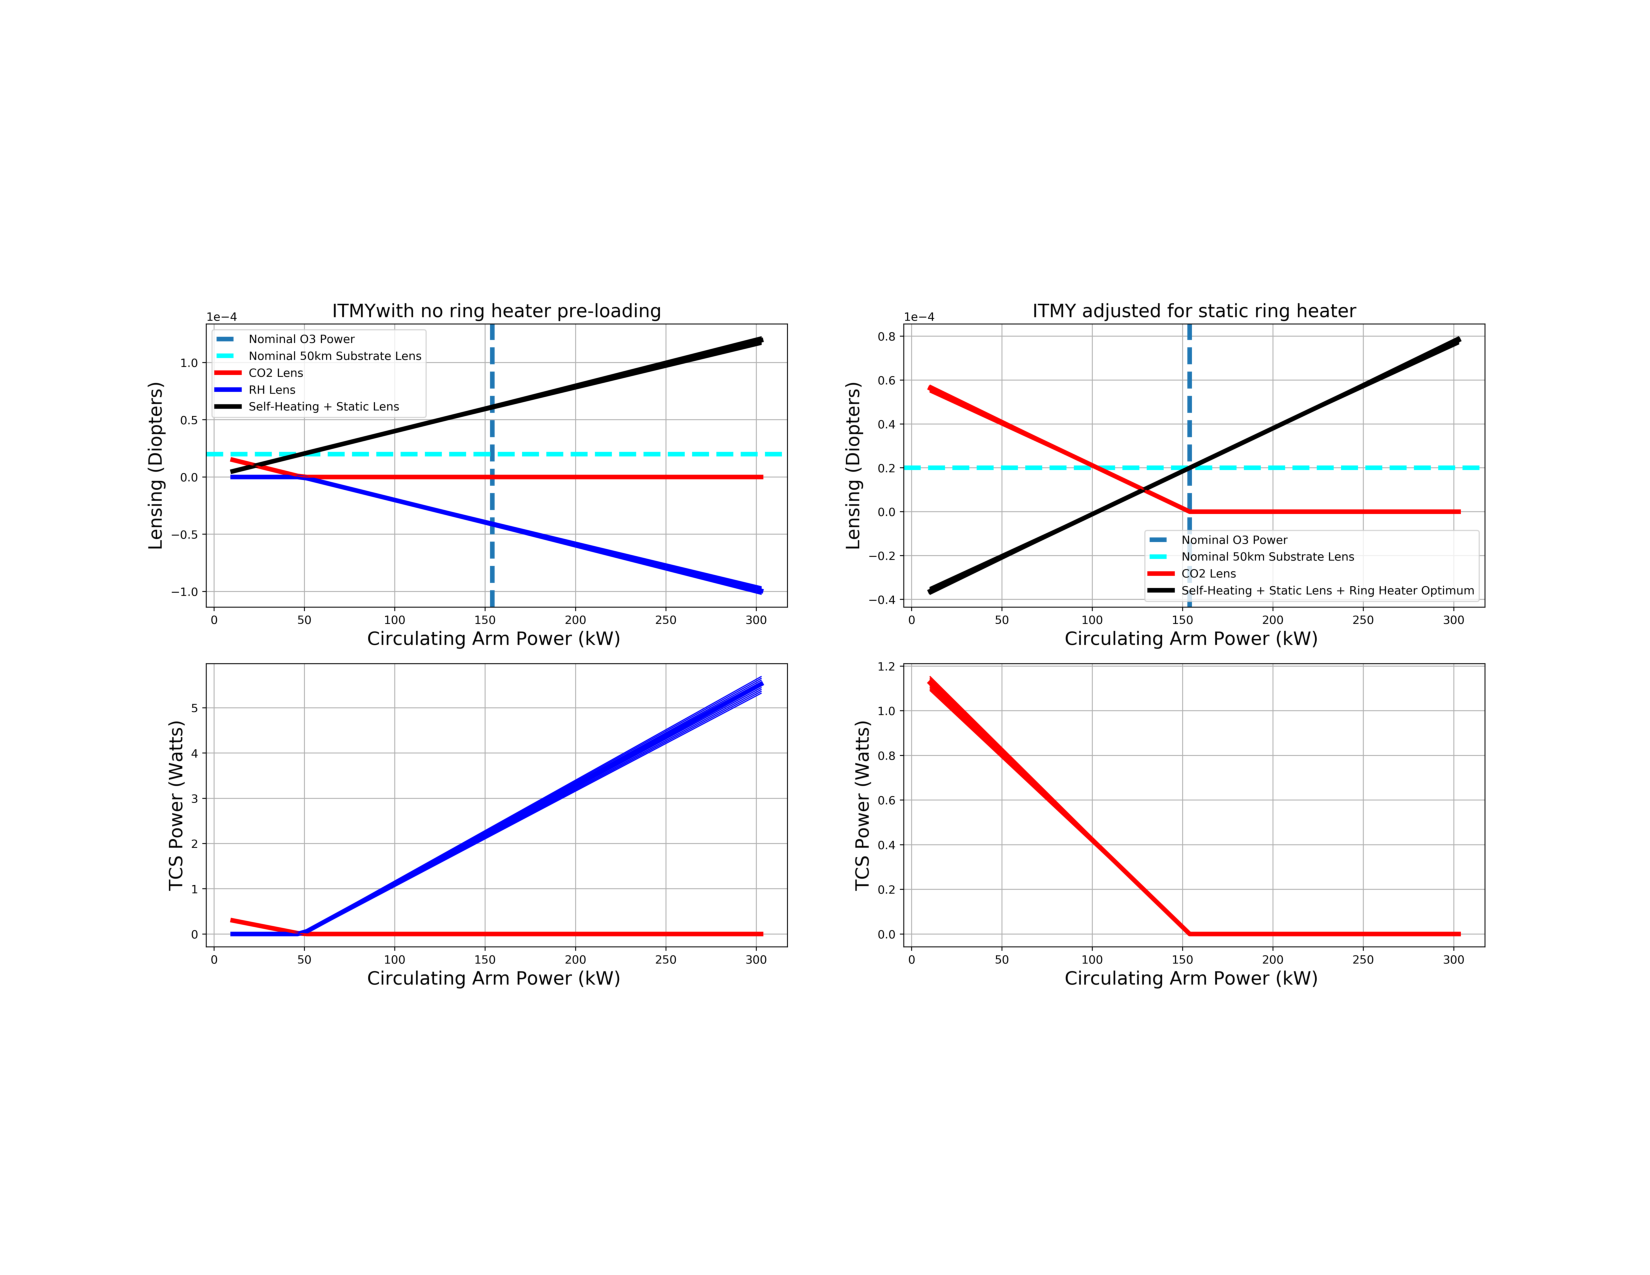
\includegraphics[width=\textwidth]{TCS/ITMY_TCS_Settings_tvo.pdf}
	  \phantomcaption\label{ITMY_TCS}
  \end{subcaptiongroup}
  \captionsetup{subrefformat=parens}
  \hfill
  \caption{The initial pre-load estimates for the ITMs at the LIGO Hanford Observatory for O3a as provided in \cite{tvo}} 
  \label{fig:O3_preload_tvo}
\end{figure}

\section{A posteriori thermal compensation for O3a}
While approaching designed arm cavity power, the presence of non-uniform absorption on the test mass coating surface imposed limits to reaching designed power and hence designed sensitivity; which simultaneously lead to a significant deviation from the original TCS pre-loading algorithm.  Assessment of these absorbers can inform methods of improving detector sensitivity required and initial characterization of these high absorbtion points which includes noting the characteristic optical path distortion as measured on the Hartmann wavefront sensors and the impacts on interferometer operations especially at high power. Current thermal actuation solutions are currently designed to control the TEM00 beam waist size and location though adjustments and modifications of current actuators was tried. This summary indicates that these absorbers may impose a barrier to maintaining high power in the arm cavities if no further proactive measures are not taken or are not sufficient to bypass detector symptoms; whether they are a result of preventable surface particulates or improved higher frequency.  

%The presence of high absorption points on the test masses (aka point absorbers) required adjustments to the TCS pre-load and various ring heater and CO2 settings were sampled. Part of this sampling lead to the development of a input ring heater filter allowing actuation to reach ? percent of the desired optical power within 2 hours compared to the 12 hour response pre-filter. Higher spatial frequency actuation in the form of a CO2 mask was also tried.

\subsection{Point absorption in O3a}
\subsubsection{ITMY absorbers}
\begin{figure}[H]
  \centering
  \begin{subcaptiongroup}
	  \includegraphics[width=.495\textwidth]{TCS/PA/ITMY_absorbers.pdf}
	  \phantomcaption\label{subfig:itmypajustself}
	  \includegraphics[width=.495\textwidth]{TCS/PA/ITMY_self.pdf}
	  \phantomcaption\label{subfig:itmypaselfplusabs}
  \end{subcaptiongroup}
  \captionsetup{subrefformat=parens}
  \hfill
  \caption{An isometric view of uniform absorption vs point absorption of LHO ITMY}
  \label{fig:ITMYpabs}
\end{figure}

\subsubsection{ETMX absorbers}
\begin{figure}[H]
  \centering
  \begin{subcaptiongroup}
	  \includegraphics[width=.49\textwidth]{TCS/PA/ETMX_absorber_short_heat.pdf}
	  \phantomcaption\label{subfig:etmxpajustself}
	  \includegraphics[width=.49\textwidth]{TCS/PA/ETMX_absorber_full_heat.pdf}
	  \phantomcaption\label{subfig:etmxpaselfplusabs}
  \end{subcaptiongroup}
  \captionsetup{subrefformat=parens}
  \hfill
  \caption{An isometric view of uniform absorption vs point absorption of LHO ETMX. The rippling / edge effects are a consequence of the Hartmann probe beam experiencing unavoidable clipping on the baffle due to misalignment of in-vaccum optics.}
  \label{fig:ETMXpabs}
\end{figure}

Impact on interferometer contrast and transmission / co-resonance of higher order modes

\subsubsection{Impacts}
A significant number of lockloss events during the comissioning period for O3A when increasing detector input power were a direct result of select optical sideband power degredation used to maintain the delicate coupled cavity configuration. And while sustaining interferometer DC readout the arm cavity would generate higher order modes sustained by Output Mode Cleaner (OMC) co-resonance; contaminating the carrier field at the output photodiode.

\paragraph{Controls schema}
\textcolor{red}{Sensor schema for interferometer control and dramatic impact to optical sidebands (higher order beat signals)}
\paragraph{Frequency noise}
\paragraph{Parasitic higher order modes}
Visible higher order modes at the anti-symmetric port \\
A significant amount of optical loss as a result of losing sideband power is reported \\
	* Lockloss caused by reduced sideband power with interferometer thermalization \\

\subsubsection{Attempted symptom reduction}
The trivial solution of reducing the test mass non-uniformity was tried but exhibited noticable limitations with the available degrees of freedom. To restore the uniformity of the test mass surface, a custom mask was constructed with the intention of imaging a negative of the optical path distortion high absorption points onto the surface with the CO2 laser combined with a static ring heater offset. 

The installation location of the mask and size was established using the relevant propogation and imaging tensors applied to the CO2 actuation field while mitigation of the aforementioned impacts provided comissioners with the notable metrics of success.

\textcolor{red}{Results}
\\
The extremely strict alignment requirement introduced difficulties while attempting to fulfill the promise of restoring uniform absorption. And although the presence of the absorber symptoms show coorelation with their prominence at high power, their collective reduction proved not to be as straightfoward~\cite{brooks:aigwd2019, buikema:2020}.
	
	* CO2 with enhanced focus on absorbers and ring heater actuation
		* Very narrow alignment requirement
		* Improvement metrics
			* Restoring sideband power	
	* Adjusting interferometer to OMC mode matching
		* Improvement metrics:
			* Reduced HOM content at detector output
			* Tracking dither line amplitudes

%\begin{figure}[H]
%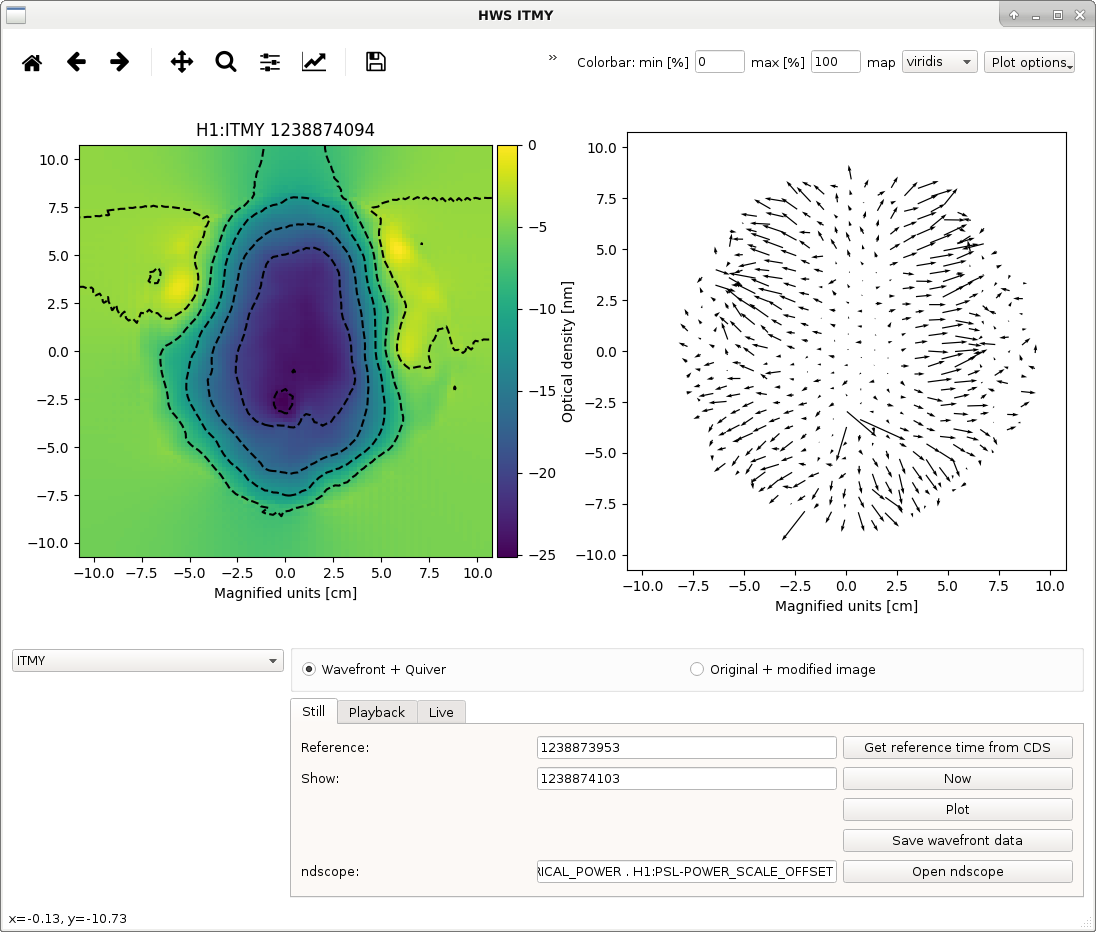
\includegraphics[width=\textwidth]{figs/TCS/PA/48349_20190409201649_inital_install_CO2Ymask2_150seconds_900mW.png}
%\caption{Point absorber figure with second $\mathrm{CO_2}$ mask}
%\label{fig:RH_power}
%\end{figure}


